\documentclass[11pt,twoside]{eitExjobb}
%%\documentclass[11pt,twoside,final]{eitExjobb}  % Use final for the final version that will be printed
%%%%%%%%%%%%%%%%%%%%%%%%%%%%%%%%%%%%%%%%%%%%%%%%%%%%
%% Other fonts (Palatino as rm font, helvetica as sf font and courier as tt font. All fonts are normally installed with a standard LaTeX distribution.)
% \usepackage{mathpazo} % Also in math mode
% \usepackage[scaled=.95]{helvet}
% \usepackage{courier}
%%%%%%%%%%%%%%%%%%%%%%%%%%%%%
% ÅÄÖ
\usepackage[utf8]{inputenc}  % Input encoding (this file): 8 bit unicode. Default by most text editors
\usepackage[T1]{fontenc}     % Output encoding (pdf file)
%%%%%%%%%%%%%%%%%%%%%%%%%%%%%
%% Packages used in the example
\usepackage{graphicx}   % Included graphics and some resizable boxes
\usepackage{url}        % nice urls with line breaks
\usepackage{indentfirst} % indent the first paragraph after section headings
\usepackage{lipsum}     % nonsense text blocks
\usepackage{amsmath}

\usepackage{float}
\usepackage{svg}
\usepackage{placeins}
\usepackage{caption}
\usepackage{xcolor}
\raggedbottom
\makeatletter
\renewcommand\chapter{\clearpage\sh@chapter}
\makeatother
%%%%%%%%%%%%%%%%%%%%%%%%%%%%%%
%%%%%%%%%%%%%%%%%%%%%%%%%%%%%%
%%%%%%%%%%%%%%%%%%%%%%%%%%%%%%
\begin{document}
%%% Title page
\Title{Efficient Mamba-Based Accelerator Architecture for Massive-MIMO Indoor Localization Using the LuViRA Dataset}
\Author{Shengjie Chen\\\texttt{sh5704ch-s@student.lu.se}\\[0.8em]Chenxi Zhang\\\texttt{ch7210zh-s@student.lu.se}}
\Supervisor{Ilayda Yaman\\Sijia Cheng}
\Examiner{Pietro Andreani}
%% Set by default
% \Date{\today}    %% Today's date
% \Year{\the\year} %% This year shown in copyright
% \Company{Department of Electrical and Information Technology\\Lund University}
%%%%%%
\MakeTitlePage  %%% Print title page and copyright page
%%%%%% 
\frontmatter    %%% Page numbering for front pages (small roman)
%%%%% Abstract
\chapter*{Abstract}
In recent years, as 6G wireless systems continue to develop, high-accuracy indoor
localization has become increasingly important for robotics, smart environments, and
location-aware services. Since indoor wireless measurements can vary over time due to
multipath propagation and environmental changes, short sequences of observations may
provide useful information for position estimation. Mamba, a sequence model based on
selective state-space updates, is therefore a promising candidate for this task because 
it can jointly process short sequences of wireless observations and
capture temporal variations in the channel.

This thesis investigates a hardware-oriented Slim-Mamba approach for Massive-MIMO indoor
localization using the LuViRA dataset. Software evaluation is first used to select a
simplified Mamba-style model that preserves the recurrent update and gating behavior
needed for localization while reducing the complexity of larger channel-fusion variants.
A Zynq MPSoC-based FPGA accelerator is then designed, with PS-side control and
PL-side input loading, four-block Slim-Mamba computation, and AXI-stream dataflow. 
We designed a shared \(4\times4\times4\) reconfigurable MAC
fabric for linear projection layers, together with a fine-grained
FIFO-based SSM(State-Space Model) pipeline to reduce waiting time between projection, nonlinear, and
state-update stages. A fixed-point quantization flow is built from Python, to bit-true
C++ modeling, and finally to RTL. 

Experimental results show that the fixed-point
implementation introduces only a small accuracy loss compared with the floating-point
model, while the FPGA accelerator meets the real-time throughput target with a clear
margin. An on-board validation test further verifies that control, memory movement,
streaming interfaces, and PL computation operate together as a complete prototype
system.
%%%%% Abstract
\chapter*{Popular Science Summary}
Finding a person or device outdoors is often easy because satellite navigation can be
used. Indoors, however, satellite signals are weak or blocked, and positioning becomes
much harder. Still, many future applications need reliable indoor positioning: a robot
may need to move safely in a building, a hospital may need to locate equipment, and a
smart environment may need to understand where people or devices are.

This thesis studies how wireless signals can be used for this purpose. When a radio
signal travels through a room, it bounces off walls, furniture, and people before it
reaches the receiver. These reflections create a kind of wireless ``fingerprint'' of the
environment. If we can learn how these fingerprints relate to positions, then a wireless
system can estimate where a device is located.

Machine learning is useful for this task because it can learn patterns that are too
complicated to describe by hand. In this work, we study a modern type of sequence model
called Mamba. A simple way to think about it is that the model does not look at one
measurement alone. Instead, it can look at a short sequence of recent measurements and
remember useful changes over time. This is promising for indoor positioning.

However, a model that works well on a computer is not automatically suitable for small
and efficient hardware. Therefore, this work is to build a hardware accelerator for 
this slim model on an FPGA, which is a programmable chip. The accelerator can be seen as a small custom
factory: data enters from memory, passes through several processing stages, and the final
position-related output is written back. To make the factory efficient, the same
calculation units are reused for several parts of the model, and the most time-critical
steps are arranged like an assembly line so that one step can start before the previous
one has completely finished.


%% ToC etc
\tableofcontents
\listoffigures
\listoftables
\clearpage
%%%%% Page numbering for the main thesis (arabic)
\mainmatter
%%%%%

\chapter{Introduction}
\section{Background}
\subsection{Indoor Localization and Massive MIMO}
\label{subsec:indoor_localization_massive_mimo}

Indoor localization is becoming an important capability for future 6G wireless
systems, since 6G is expected to support not only ubiquitous communication but
also high-accuracy localization and high-resolution sensing
services~\cite{cite:Bourdoux2020}. Localization is also regarded as a key
enabler for future 6G wireless systems~\cite{cite:Trevlakis2023}. With the
development of location-aware applications such as robotic navigation,
emergency healthcare, and smart transportation, wireless localization is
expected to support a wider range of location-aware
services~\cite{cite:Tian2024}. At the same time, real-time indoor positioning
has long remained a challenging problem~\cite{cite:Mogyorosi2022}. In indoor
wireless localization systems, localization performance is affected by
environmental factors such as multipath and non-line-of-sight propagation,
which makes accurate positioning challenging~\cite{cite:Yaro2023}.

In this context, massive multiple-input multiple-output (Massive MIMO) provides
a promising measurement platform for radio-based indoor localization. By
equipping the base station with a large antenna array, Massive MIMO provides
rich spatial channel observations that can be exploited for localization.
Previous work has used the instantaneous spatial covariance matrix to capture
angular information and the channel impulse response to capture delay
information~\cite{cite:TianICC2023}. These angular-domain and delay-domain
features are useful because they provide complementary descriptions of the
location-dependent radio channel in complex indoor environments. Therefore,
Massive MIMO can provide favorable conditions for high-precision indoor
positioning by enabling location-dependent channel information to be extracted
from measured radio signals~\cite{cite:TianICC2023}.

Figure~\ref{fig:lumami_setup} illustrates a representative Massive-MIMO-based
indoor localization setup. A user equipment (UE) or mobile platform moves inside
the measurement area, while a base-station antenna array records the radio
channel from different positions. As the UE moves, the propagation paths and the
measured channel response change with its location, which makes the radio
measurement useful as a position-dependent fingerprint.

\begin{figure}[H]
  \centering
  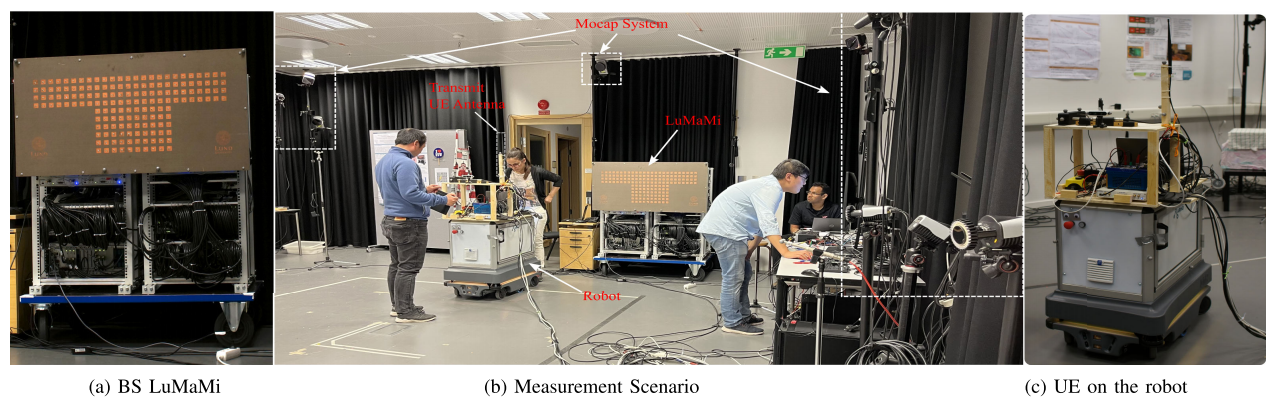
\includegraphics[width=0.90\linewidth]{lumami.png}
  \caption{Massive MIMO indoor localization measurement setup with moving user equipment, adapted from~\cite{cite:Tian2024}.}
  \label{fig:lumami_setup}
\end{figure}

However, Massive MIMO provides high-dimensional spatial channel
measurements, while the final positioning accuracy still depends on how the
channel information is represented and how the localization model extracts
useful features from it.

\subsection{Radio-Based Positioning Methods}
\label{subsec:radio_positioning_methods}

Radio localization estimates the position of a user equipment or mobile platform
from measured wireless channel information. In the LuViRA dataset, the radio
modality is described as the channel response between a 5G massive
multiple-input multiple-output testbed and user equipment~\cite{cite:LuViRA2024}.
The localization system uses radio measurements whose values depend on the
relative position between the transmitter, the receiver array, and the
surrounding indoor environment. Since the radio channel changes with the
position of the transmitter, these measured channel responses can be used as
location dependent fingerprints for positioning.

For localization with Massive MIMO, previous work roughly classifies the
methods into three groups: methods based on angle estimation, methods based on
position estimation, and methods based on fingerprinting~\cite{cite:Tian2024}.
Traditional angle estimation and position estimation methods usually rely on
explicit geometric or signal processing assumptions, while fingerprinting and
learning based methods use measured channel features as position related
signatures. In the LuViRA setting, the radio measurements are collected in a
realistic indoor environment, where a transmit antenna is mounted on a moving
service robot and the channel response is recorded together with accurate ground
truth pose labels~\cite{cite:LuViRA2024}. This provides paired data between
radio channel measurements and position labels, which can be used to train
supervised fingerprinting or regression models for localization.

Machine learning naturally extends this fingerprinting idea by learning the
mapping from channel observations to user positions from data. In this
formulation, ML models take radio channel fingerprints as inputs and estimate
the localization of the user equipment. This is
attractive for Massive MIMO indoor localization because the measured channel
contains rich spatial and delay information that may be difficult to fully
represent using explicit geometric or model based assumptions. Previous work
has also shown that multiple processing chains can be trained with different
channel fingerprints and then combined to improve localization
performance~\cite{cite:Tian2024}.

\subsection{LuViRA Radio Dataset Used in This Thesis}
\label{subsec:luviva_radio_dataset}

The experimental data used in this thesis are taken from the radio modality of
the Lund University Vision, Radio, and Audio (LuViRA) dataset. LuViRA is a
synchronized multi-sensor dataset for indoor localization, including color
images, depth maps, inertial measurement unit readings, radio channel responses,
audio recordings, and accurate six-degree-of-freedom ground truth pose
measurements~\cite{cite:LuViRA2024}. Although the full dataset contains several
sensing modalities, this thesis focuses only on the grid data from the radio
measurements, since the target application is Massive MIMO indoor localization.

In the radio part of LuViRA, the measured data are described as the channel
response between a 5G massive multiple-input multiple-output testbed and user
equipment~\cite{cite:LuViRA2024}. In the measurement setup, a transmit antenna
is mounted on a slowly moving service robot together with the other
sensors~\cite{cite:LuViRA2024}. Therefore, the object localized in this thesis
is the moving platform, represented by the radio transmitter mounted on the
robot. The ground truth position is provided by the motion capture system, which
is used to verify the localization results obtained from the sensor
measurements~\cite{cite:LuViRA2024}.

The LuViRA dataset contains 89 recorded trajectories, and each trajectory
includes approximately 20 to 50 seconds of synchronized sensor data and ground
truth labels~\cite{cite:LuViRA2024}. In this thesis, however, the full
multi-modal dataset is not used. Only the radio grid data are used as model
inputs, while the corresponding ground truth positions are used as supervision
during training and as reference labels for evaluating localization error. An
example of the grid trajectory layout used in the LuViRA radio measurements is
shown in Fig.~\ref{fig:luviva_grid_trajectory}.

\begin{figure}[H]
  \centering
  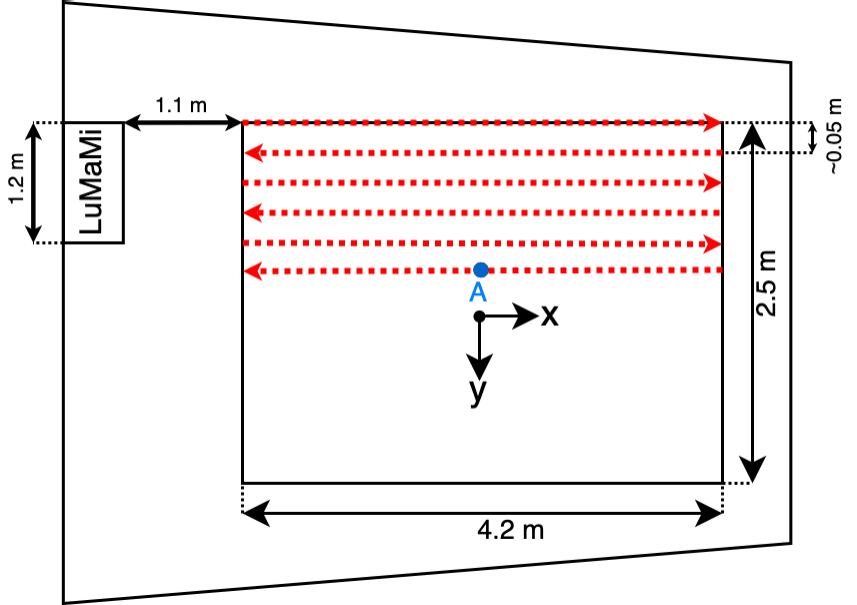
\includegraphics[width=0.65\linewidth]{trajectory.png}
  \caption{Example grid trajectory layout in the LuViRA radio dataset, adapted from~\cite{cite:Tian2024}.}
  \label{fig:luviva_grid_trajectory}
\end{figure}

The dataset used in this work is divided into three non-overlapping subsets:
training, evaluation, and test. Following the same data split strategy as the
FCNN baseline used for comparison~\cite{cite:TianICC2023,cite:Tian2024}, the
test set and the training/evaluation pool are separated according to the parity
of the grid index. The even-grid data are used as the test set, while the
odd-grid data are used as the training and evaluation pool. The evaluation set
is then formed by randomly selecting two groups from the odd-grid data, and the
remaining odd-grid data are used for training.

This split keeps the training, evaluation, and test sets separated at the grid
level while following the same experimental setting as the FCNN baseline. As a
result, the proposed Mamba based models and the previous FCNN based method can
be compared under a consistent data partition, making differences in localization
accuracy more attributable to the model design rather than to different dataset
splits.

\section{Related Work}
In recent years, machine learning has been investigated for Massive-MIMO-based indoor
localization. Tian et al. proposed FCNN-based localization methods that use spatial
covariance matrices and truncated channel impulse responses to capture angular- and
delay-domain information, achieving centimeter-level accuracy in indoor Massive MIMO
measurements~\cite{cite:TianICC2023}. Their later work further introduced an ML-based
localization pipeline with multiple processing chains and ensemble learning to fuse
different channel fingerprints~\cite{cite:Tian2024}. However, these studies also show
that network training and fine tuning can become challenging due to the
increase in network size~\cite{cite:Tian2024}.
Although subarray-based processing can reduce network size, efficient and
hardware-friendly model design remains an important issue for practical
deployment~\cite{cite:Tian2024}.

However, most existing ML-based Massive MIMO indoor localization methods rely on
FCNNs~\cite{cite:Tian2024}, CNNs~\cite{cite:Colpaert2023},
KNN~\cite{cite:Cunningham2022KNN}, or other conventional machine-learning models to
process high-dimensional channel fingerprints. These methods can effectively exploit
channel features, but for densely connected models such as FCNNs, higher-dimensional
inputs usually lead to larger network sizes, more parameters, and higher training and
inference cost. Existing work also points out that, when ML-based localization methods
are applied to Massive MIMO systems, the increase in network size can make training and
fine-tuning more challenging~\cite{cite:Tian2024}. Therefore, reducing model size,
computational complexity, and hardware deployment cost while maintaining localization
accuracy remains an important research problem in Massive-MIMO-based indoor
localization.


\section{Goals and Challenges}
The goal of this thesis is to investigate the efficiency of Mamba-like architectures
for Massive-MIMO indoor localization and further explore their FPGA-based hardware
acceleration. Mamba is a selective state-space sequence model that uses input-dependent
state updates to selectively propagate or forget information along the sequence
dimension, while maintaining linear scaling with sequence length~\cite{cite:Mamba2023}.
This property makes Mamba attractive for continuous wireless measurement sequences,
because it uses recurrent state updates without the parameter explosion commonly
associated with FCNNs when the input dimension increases.

Compared with previous FCNN-based methods that mainly operate on single snapshots or
fixed fingerprints, Mamba can process short sequences of observations jointly and
exploit temporal dynamics in the wireless channel. Therefore, this thesis aims to
evaluate Mamba-family models for LuViRA indoor localization, design a hardware-friendly
slim Mamba-like architecture, and implement the key Mamba datapath on FPGA with
quantization-aware considerations. The main challenges include preserving localization
accuracy after model simplification and quantization, handling the memory and
computation pressure caused by high-dimensional CSI, and balancing latency, power,
resource utilization, and localization accuracy in the final accelerator design. Recent
studies have explored Mamba acceleration in other application scenarios, including
FPGA-based quantization and hardware co-design with computation reordering and
fine-grained tiling, pipelined vector processing units, and hybrid dataflows with
state-space buffers~\cite{cite:LightMamba2025,cite:FastMamba2025,cite:HCSA2025}.
Motivated by these works, this thesis further investigates how the Slim Mamba datapath
can be reused for indoor localization, with particular attention to datapath reuse,
memory access organization, and pipeline granularity.


\chapter{Algorithm}

\section{Mamba Basics}
Mamba is a sequence modeling architecture based on selective state-space models
(selective SSMs). A state-space model represents historical information using a hidden
state and describes the dynamics of an input sequence through state transitions. A
continuous-time state-space model can be written as
\begin{equation}
\dot{h}(t)=Ah(t)+Bx(t),
\end{equation}
\begin{equation}
y(t)=Ch(t)+Dx(t),
\end{equation}
where $x(t)$ is the input, $h(t)$ is the hidden state, and $y(t)$ is the output. The
matrix $A$ controls the state dynamics, $B$ determines how the input affects the state,
$C$ maps the hidden state to the output, and $D$ represents a direct input-to-output
path. To process discrete sequences, the continuous system can be discretized into a
recurrent form:
\begin{equation}
h_t=\bar{A}_t h_{t-1}+\bar{B}_t x_t,
\end{equation}
\begin{equation}
y_t=C_t h_t+D x_t,
\end{equation}
where $x_t$ is the input at time step $t$, $h_t$ is the current hidden state, and $y_t$
is the current output. The discretized parameters can be written as
\begin{equation}
\bar{A}_t=\exp(\Delta_t A),
\end{equation}
\begin{equation}
\bar{B}_t=(\Delta_t A)^{-1}\left(\exp(\Delta_t A)-I\right)\Delta_t B_t.
\end{equation}

The key idea of Mamba is to make part of the SSM parameters input-dependent. For
example, $\Delta_t$, $B_t$, and $C_t$ can be generated from the current input $x_t$
through lightweight linear projections. In this way, the model can dynamically decide
what information should be preserved, updated, or forgotten according to the current
input. Gu and Dao show that making SSM parameters functions of the input allows the
model to selectively propagate or forget information along the sequence dimension,
while Mamba maintains linear scaling with sequence length~\cite{cite:Mamba2023}.


From an architectural perspective, a Mamba block usually consists of an input
projection, local feature mixing, a selective scan, a gating branch, and an output
projection. The input is first projected and split into a main branch and a gate
branch. The main branch generates the dynamic SSM parameters and updates the hidden
state through the selective scan. The gate branch is usually passed through a nonlinear
activation function such as SiLU and then multiplied with the SSM output, followed by
an output projection. Since the state update can be implemented recurrently over time,
Mamba can model contextual information with low sequence complexity and avoids the
quadratic complexity commonly associated with attention-based methods on long
sequences~\cite{cite:Mamba2023}.


Mamba is worth investigating for indoor localization because indoor wireless
measurements can often be organized as user trajectories or consecutive channel
snapshots, where neighboring snapshots may contain short-term contextual information
useful for position estimation. Compared with FCNN-based methods that mainly operate on
single snapshots or fixed channel fingerprints, Mamba can progressively aggregate
historical observations through its recurrent state and adaptively update the state
according to the current input. Therefore, Mamba provides a model candidate that can
exploit temporal context while maintaining linear sequence complexity, making it
suitable for further investigation in terms of accuracy, efficiency, and hardware
implementation for Massive-MIMO-based indoor localization.


\section{Slim-Mamba}
\label{sec:slim_mamba}
In this work, Slim Mamba is designed as a lightweight Mamba variant for
Massive-MIMO-based indoor localization. The model is not obtained by directly adopting
the original Mamba architecture, but rather through a task-driven simplification
process based on preliminary model exploration. The initial design followed a
channel-aware Mamba direction, where multi-branch structures were used to fuse
different types of radio features, such as the real and imaginary parts of the channel
impulse response (CIR), power features, and first-order difference features. A similar
motivation can be found in CMamba, where vanilla Mamba is considered insufficient for
modeling cross-channel dependencies in multivariate time series, and additional
channel-correlation modeling is introduced to enhance interactions among different
channels~\cite{cite:CMamba2024}. For the LuViRA indoor localization task, different
radio-domain features may also contain complementary location-related information,
making channel-fusion design a reasonable initial direction.

However, preliminary experiments showed that the additional channel-fusion branches
provided only limited accuracy improvement for the current localization task, while
significantly increasing model size, training time, and hardware mapping complexity. At
the same time, the vanilla Mamba v1 baseline, implemented following the original Mamba
architecture proposed by Gu and Dao~\cite{cite:Mamba2023}, showed a clear
generalization gap on LuViRA, whereas short temporal windows were already sufficient to
provide useful localization information. Therefore, the final model follows a
task-driven simplification principle: it preserves the recurrent state update and
input-dependent modulation mechanisms that are most relevant to the localization task,
while removing complex multi-branch fusion structures and the full selective-scan
parameterization.


Table~\ref{tab:model_variants} summarizes the measured comparison among the FCNN
baseline, channel mamba, vanilla Mamba v1, and slim mamba on the LuViRA dataset.
Compared with channel mamba, slim mamba achieves a comparable test mean error while
reducing the model size from 40.4~MB to 3.40~MB and the training time from 73~s to 13~s
per epoch. Compared with vanilla Mamba v1, slim mamba significantly improves
localization accuracy while maintaining a similarly compact model size. These results
indicate that slim mamba provides a better trade-off among localization accuracy, model
complexity, training efficiency, and hardware cost for the target indoor localization
task.


\begin{table}[!htbp]
  \centering
  \caption{Comparison of results on different models.}
  \label{tab:model_variants}
  \resizebox{\linewidth}{!}{%
  \begin{tabular}{lcccccc}
    \hline
    Model & Input & Size & Time & it/s & Err. & HW Cost \\
          & Features & (MB) & (s/epoch) & & (cm) & Proxy \\
    \hline
    FCNN & CIR & 440 & N/A & N/A & $\sim$13 & High \\
    channel mamba & CIR + Power & 40.4 & 73 & 13.18 & 12.9 & High \\
    Vanilla Mamba v1 & CIR + Power & 3.38 & 33 & 32.62 & 24.74 & Medium \\
    slim mamba & CIR + Power & 3.40 & 13 & 75.30 & 13.5 & Low \\
    \hline
  \end{tabular}%
}
\end{table}

\FloatBarrier

As illustrated in Fig.~\ref{fig:slim_mamba}, the Slim Mamba block first applies
normalization to the input tokens, followed by a linear input projection that maps the
input into an internal feature space. The projected representation is then split into
two paths: a state input branch and a gate branch. The state input branch is used for
state-space model (SSM) state updating, while the gate branch is used for output
modulation.


\begin{figure}[H]
  \centering
  \includesvg[width=0.70\linewidth]{ssm_block_flownew}
  \caption{Simplified datapath of the Slim Mamba block.}
  \label{fig:slim_mamba}
\end{figure}

\FloatBarrier

In the state input branch, the update gate generator produces an input-dependent update
coefficient $\lambda_t$ from the current state input:
\begin{equation}
\lambda_t = \sigma(W_{\lambda} * u_t + b_{\lambda}),
\label{eq:slim_mamba_lambda_conv}
\end{equation}
where $*$ denotes the convolution operation, $\sigma(\cdot)$ is the sigmoid function,
and $\lambda_t$ is constrained to the range $(0,1)$ so that it can control the
interpolation between the previous state and the current input. The recurrent state
update is computed as
\begin{equation}
s_t = \lambda_t \odot s_{t-1} + (1-\lambda_t) \odot u_t,
\label{eq:slim_mamba_state_update}
\end{equation}
where $s_{t-1}$ is the previous state, $u_t$ is the current state input, and
$\lambda_t$ is the update gate that controls the balance between the historical state
and the current input. When $\lambda_t$ is fixed, this recurrence is equivalent to an
exponential moving average, since older inputs receive weights that decay as powers of
$\lambda$. In Slim Mamba, however, $\lambda_t$ is dynamically generated from the
current input, and the module is therefore more accurately described as an
input-dependent gated state update. Compared with the full $(A,B,C,D)$ selective-scan
parameterization and low-rank discretization in the original Mamba, this formulation
leads to a more regular computation path and is more suitable for hardware
implementation~\cite{cite:Mamba2023}.

In parallel, the gate branch is passed through a SiLU activation to generate the output
gate:
\begin{equation}
g_t = \mathrm{SiLU}(v_t).
\label{eq:slim_mamba_output_gate}
\end{equation}
The output gate then modulates the updated state through element-wise multiplication:
\begin{equation}
z_t = s_t \odot g_t.
\label{eq:slim_mamba_output_modulation}
\end{equation}
This gating operation allows the model to regulate the effective information from the
SSM output according to the current input. The result is then passed through a linear
output projection and added back to the input tokens through a residual connection. The
residual path helps preserve the original input information and improves training
stability. Overall, Slim Mamba retains the recurrent state update and gated modulation
mechanisms of Mamba, while removing complex channel-fusion branches that provide
limited benefit for the current task.

Compared with channel mamba, Slim Mamba adopts a single-path backbone and reduces
branch control and cross-channel fusion overhead. Compared with vanilla Mamba, it
simplifies the state-update parameterization and concentrates the main computation on
regular operators such as linear projection, update gate generation, state update,
element-wise multiplication, and output projection. This structure is more suitable for
pipelined FPGA implementation and fixed-point quantization, and provides a clear
datapath foundation for the subsequent Mamba-based indoor localization accelerator.


\chapter{Method}

\section{Hardware Architecture}
This section presents the overall hardware architecture of the Slim-Mamba FPGA
accelerator. The design is deployed on a Zynq MPSoC platform, where the processing
system (PS) handles software control and DDR management, while the programmable logic
(PL) implements the accelerator datapath. The PS-side DDR4 is used as off-chip runtime
storage for input and output buffers. The input vector $x_t$ is read from DDR through
the memory-mapped to stream (MM2S) channel of the AXI DMA and sent to the PL as an
AXI-Stream. The output $y_t$ is written back to DDR through the stream to memory-mapped
(S2MM) channel. The PS configures the accelerator through AXI-Lite control/status
registers, including input preload, computation start, status polling, and interrupt
control.

\begin{figure}[H]
  \centering
  \includesvg[width=0.9\linewidth]{tcas_hardware_architecture}
  \caption{Diagram of Slim-Mamba overall hardware architecture.}
  \label{fig:tcas_hardware_architecture}
\end{figure}

Inside the PL, the board shell connects the external AXI interfaces to the compute
pipeline formed by four Slim-Mamba blocks. The AXI-Lite CSR first starts the input
stream loader, which writes the incoming AXI-Stream data into the on-chip input buffer
of the first block. After the preload stage is completed, the shell allows the 4-block
controller to start computation. The controller schedules the four blocks sequentially.
Between adjacent blocks, the output of the current block is added to the residual using
saturated fixed-point arithmetic and then preloaded into the input buffer of the next
block. The final block output is not passed through another block-level residual
preload stage, but is directly streamed to the DMA as $y_t$.


Within each Slim-Mamba block, the main MAC-intensive stages share a reconfigurable MAC
fabric. The input projection scheduler, the $\Delta$ projection scheduler, and the
output projection scheduler generate tiled operands from on-chip weight and activation
buffers. The MAC fabric manager selects the active scheduler and sends its operands to
the shared $4\times4\times4$ MAC fabric. This fabric consists of four $4\times4$ PE
arrays. By time-multiplexing the same fabric across different projection stages, the
design avoids instantiating separate MAC arrays and reduces DSP and on-chip
interconnect cost.


The design also uses a unified reconfigurable quantization stage. After MAC or
element-wise computation, intermediate results are scaled, rounded, and saturated
according to the current scheduler and datapath mode, and are then mapped back to the
target fixed-point format. Therefore, the same quantization module can support
different scale parameters across projection stages and element-wise operations. In the
current implementation, weights, scale parameters, and nonlinear lookup tables are
initialized into on-chip PL memories through memory initialization files, while DDR is
mainly used for runtime input and output data movement.


\section{Linear Layers}
\label{subsec:linear_layer_mac_array}


As discussed in Section~\ref{sec:slim_mamba}, the Slim Mamba algorithm can be mapped to
three major hardware primitives. The first primitive is matrix-vector multiplication
(MVM) implemented with multiply-accumulate (MAC) operations, which is mainly used for
the input projection, the update-gate projection(dt projection), and the output
projection. The second primitive is element-wise multiplication, or EWM, which is used
for the weighted terms in the state update and for output gating. The third primitive is
element-wise addition, or EWA, which is used for the state update and residual addition.
In the SSM datapath, these three primitives correspond to the projection computation,
the recurrent state update, and the output gating operation, respectively.

\subsection{Reuse vs.\ Latency Trade-off}
From a hardware design perspective, these primitives can be mapped with different
resource-reuse strategies. One option is to build a unified reconfigurable PE array,
where the processing elements switch among MAC, EWM, and EWA modes through a common
mode signal. This approach maximizes the reuse of multipliers, adders, and local
buffers, thereby reducing area and resource cost. However, since different computation
stages share the same array, this design may introduce mode-switching overhead,
scheduling stalls, and a coarser pipeline granularity. Another option is to map the
projection-heavy computations to a shared MAC fabric, while using lightweight vector
EWM/EWA modules for state update and output gating. This design introduces some
additional resources, but it allows projection, state update, and output gating to be
connected in a finer-grained streaming pipeline.


Therefore, the current implementation adopts a compromise between resource reuse and
pipeline granularity. The underlying PE array is capable of supporting MAC, EWM, and
EWA modes through a unified mode signal. In the current Slim Mamba accelerator,
however, the input projection, dt projection, and output projection paths mainly use
the shared MAC fabric in MAC mode. The element-wise multiply/add operations in the SSM
state update and the element-wise multiplication in output gating are implemented using
dedicated vector modules. In other words, the design preserves the reconfigurable
capability of MAC/EWM/EWA execution, but functionally separates projection computation
from element-wise computation to achieve better pipeline granularity and module
decoupling.


This choice is also reflected in the fine-grained scheduling of the SSM datapath. In a
coarse-grained design, different stages tend to execute sequentially, which improves
resource reuse but increases end-to-end waiting time. In contrast, fine-grained
streaming allows each MAC tile to be forwarded immediately to the following state
update and output gating stages. In our throughput analysis with $N=64$ tiles, the
fine-grained schedule reduces latency from
\begin{equation}
T_A = 29N
\label{eq:coarse_latency}
\end{equation}
to
\begin{equation}
T_B = 22N + 7,
\label{eq:fine_latency}
\end{equation}
that is, from 1856 cycles to 1415 cycles, corresponding to a 23.8\% reduction. This
schedule adds only about 12 DSPs per SSM compute path, which is acceptable compared
with the achieved latency reduction. Based on this trade-off, the design adopts a
fine-grained FIFO-based AXI-stream control scheme instead of relying entirely on a
single reconfigurable array for all computations.

\subsection{MAC Array Architecture Selection}

The core workload of the linear layers can be abstracted as matrix-vector
multiplication. Taking the dt projection as an example, its linear part can be
expressed as
\begin{equation}
a_t = W_{\lambda}u_t + b_{\lambda},
\label{eq:update_gate_projection_linear}
\end{equation}
where $u_t$ is the state input, and $W_{\lambda}$ and $b_{\lambda}$ are the projection
weight and bias, respectively. This computation is performed by the MAC fabric.
Similarly, the input projection generates the state input and gate input from the input
feature, while the output projection maps the gated result back to the block output
dimension. These projections are all MAC operations and can therefore reuse the same
MAC fabric with different input buffers, weight buffers, and output destinations.

Take SSM projection workload for example, a typical linear layer can be modeled as the
multiplication between a $256\times256$ matrix and a $256\times1$ vector, resulting in
\begin{equation}
256 \times 256 = 65,536
\label{eq:total_mac_ops}
\end{equation}
MAC operations. Given a fixed number of processing elements, the ideal lower bound of
the compute cycles can be estimated by
\begin{equation}
CC_{\min} =
\left\lceil
\frac{\text{Total MAC operations}}{\#\text{PEs}}
\right\rceil .
\label{eq:cc_min}
\end{equation}
This formula only gives a theoretical lower bound. The actual latency is also affected
by pipeline fill and drain, reduction, scheduling, and data delivery. Based on this
workload, three candidate MAC array organizations are compared in
Table~\ref{tab:mac_array_tradeoff}. Here, the number of ``+'' symbols qualitatively
indicates the relative wiring complexity.

\begin{table}[t]
\centering
\caption{Comparison of candidate MAC array organizations for projection computation.}
\label{tab:mac_array_tradeoff}
\resizebox{\linewidth}{!}{%
\begin{tabular}{lccc}
\hline
 & $16\times16$ Systolic & $64\times1$ GEMV & $4\times4\times4$ Pipeline \\
\hline
Wires & +++ & + & ++ \\
DSPs & 256 & 64 & 64 \\
BW (weights/cycle) & 256 & 64 & 64 \\
Clock cycles for $(256,256)$ MVM & 256 & 1024 & 1024 \\
\hline
\end{tabular}%
}
\end{table}

A large $16\times16$ systolic array provides high spatial parallelism and a low
theoretical cycle count. However, for the projection workload in this design, the
computation is dominated by GEMV rather than large-batch GEMM. Therefore, the
two-dimensional data reuse advantage of a large systolic array is not fully exploited,
while the larger PE scale introduces higher global routing, control, and data-supply
pressure.


A $64\times1$ GEMV engine is more directly matched to matrix-vector multiplication.
However, in a typical $64\times1$ GEMV engine, if all 64 MACs serve one output lane, 64
products are generated in one cycle and must be reduced into one partial sum for that
output channel. This usually requires a 64-input adder tree, or a multi-stage pipelined
adder tree. Although such a structure is suitable for pure GEMV computation, the large
adder-tree fan-in may increase the number of adder stages, routing complexity, and the
pressure of pipeline register insertion, making timing closure more challenging on
FPGA.


The proposed $4\times4\times4$ MAC array organizes the 64 PEs as four cascaded
$4\times4$ sub-arrays. Each sub-array processes a small input-weight tile, while the
four sub-arrays are activated with a staggered schedule to combine local spatial
parallelism and inter-array pipelining. The comparison above shows the advantage of
this organization. Compared with a $64\times1$ GEMV engine, it provides higher
vector-output parallelism and reduces the pressure of a large top-level reduction
tree. Compared with a large $16\times16$ systolic array, it avoids excessive global
routing and data-supply pressure for the MVM-dominated workload. Therefore, the
$4\times4\times4$ structure is selected as a balanced shared MAC fabric in terms of
resource cost, pipeline regularity, and timing closure.


At each cycle, a sub-array receives a 4-element slice of the input vector together
with a $4\times4$ weight block. The first sub-array starts a new output tile, and
the following sub-arrays join the same tile with a one-cycle offset. Weights are
scheduled in 4-column blocks. For each sub-array, the column start index advances
by a fixed stride of 16 every cycle, as summarized in
Table~\ref{tab:col_progress}. Within the same cycle, the four sub-arrays access
distinct column blocks with fixed offsets \(\{0,4,8,12\}\), resulting in a
constant 12-column spacing between adjacent active arrays, as shown in
Table~\ref{tab:col_spacing}.

\begin{table}[H]
\centering
\setlength{\abovecaptionskip}{2pt}
\setlength{\belowcaptionskip}{0pt}
\begin{minipage}[t]{0.47\linewidth}
\centering
\captionof{table}{Column starts per sub-array.}
\label{tab:col_progress}
\small
\setlength{\tabcolsep}{4pt}
\resizebox{\linewidth}{!}{%
\begin{tabular}{c|l|c}
\hline
\textbf{Array} & \textbf{Column Start Points} & \textbf{$\Delta$} \\
\hline
Array1 & 0 $\rightarrow$ 16 $\rightarrow$ 32 $\rightarrow$ 48 $\rightarrow$ 64 & +16 \\
Array2 & 4 $\rightarrow$ 20 $\rightarrow$ 36 $\rightarrow$ 52 & +16 \\
Array3 & 8 $\rightarrow$ 24 $\rightarrow$ 40 & +16 \\
Array4 & 12 $\rightarrow$ 28 & +16 \\
\hline
\end{tabular}%
}
\end{minipage}
\hfill
\begin{minipage}[t]{0.50\linewidth}
\centering
\captionof{table}{12-column array spacing.}
\label{tab:col_spacing}
\small
\setlength{\tabcolsep}{4pt}
\renewcommand{\arraystretch}{1.12}
\resizebox{\linewidth}{!}{%
\begin{tabular}{c|c|c|c}
\hline
\textbf{Cycle} & \textbf{A1$\rightarrow$A2 $\Delta$} &
\textbf{A2$\rightarrow$A3 $\Delta$} & \textbf{A3$\rightarrow$A4 $\Delta$} \\
\hline
2 & 16--4 = \textbf{12} & -- & -- \\
3 & 32--20 = \textbf{12} & 20--8 = \textbf{12} & -- \\
4 & 48--36 = \textbf{12} & 36--24 = \textbf{12} & 24--12 = \textbf{12} \\
5 & 64--52 = \textbf{12} & 52--40 = \textbf{12} & 40--28 = \textbf{12} \\
\hline
\end{tabular}%
}
\end{minipage}
\end{table}

Also, the input vector $x_t$ follows the same staggered
pipeline as the weight tiles. Each sub-array receives the activation slice that
matches its current $4\times4$ weight block, and these slices are delayed together
with the corresponding weights to keep the four sub-arrays aligned. After the 16
column groups of the current output-row tile have been consumed, the scheduler
switches to the next output-row tile. Table~\ref{tab:mac_pipeline_schedule}
illustrates this tile-switching pattern.


\begin{table*}[!t]
\caption{Weight input scheduling for the pipelined MAC arrays.}
\label{tab:mac_pipeline_schedule}
\centering
\small
\setlength{\tabcolsep}{3pt}
\resizebox{\textwidth}{!}{%
\begin{tabular}{c|l|l|l|l|l}
\hline
\textbf{Cycle} & \textbf{Array1 Columns} & \textbf{Array2 Columns} & \textbf{Array3 Columns} & \textbf{Array4 Columns} & \textbf{Description} \\
\hline
1  & col0--3   & -- & -- & -- & ARRAY1 preloads first $4\times4$ block (tile1). \\
2  & col16--19 & col4--7 & -- & -- & ARRAY2 begins tile1. \\
3  & col32--35 & col20--23 & col8--11 & -- & ARRAY3 begins tile1 (3-cycle stagger). \\
4  & col48--51 & col36--39 & col24--27 & col12--15 & ARRAY4 joins; pipeline full. \\
5--16 & continue +16 stride & same & same & same & Steady-state loading of tile1. \\
17 & {\color{blue}\textbf{col256--259 $\rightarrow$ tile2}} & col244--247 & col232--235 & col220--223 & \textbf{ARRAY1 starts tile2 (row4--7).} \\
18 & col272--275 & {\color{blue}\textbf{col260--263 $\rightarrow$ tile2}} & col248--251 & col236--239 & \textbf{ARRAY2 switches to tile2.} \\
19 & col288--291 & col276--279 & {\color{blue}\textbf{col264--267 $\rightarrow$ tile2}} & col252--255 & \textbf{ARRAY3 switches to tile2.} \\
20 & col304--307 & col292--295 & col280--283 & {\color{blue}\textbf{col268--271 $\rightarrow$ tile2}} & \textbf{ARRAY4 switches; tile1 finishes.} \\
21--37 & continue +16 stride & same & same & same & Steady-state operation for tile2. \\
38 & {\color{red}\textbf{tile3 preload}} & -- & -- & -- & ARRAY1 starts tile3. \\
39 & -- & {\color{red}\textbf{tile3 preload}} & -- & -- & ARRAY2 starts tile3. \\
40 & -- & -- & {\color{red}\textbf{tile3 preload}} & -- & ARRAY3 starts tile3. \\
41 & -- & -- & -- & {\color{red}\textbf{tile3 preload}} & ARRAY4 starts tile3 (3-cycle stagger). \\
42--58 & continue +16 stride & same & same & same & Steady tile3 operation. \\
\hline
\end{tabular}%
}
\end{table*}

\subsection{Hardware Implementation of Linear Layers}

An example of the array hardware implementation is shown in
Fig.~\ref{fig:tcas_hardware_architecture}(d). Local accumulation is first performed
inside the $4\times4$ MAC arrays, and the partial results generated by the four
sub-arrays are then sent to a 4-input reduction tree to form the vector output. The
reduced vector does not need to wait for all later partial vectors of the layer to be
completed. Instead, it is forwarded through FIFO interfaces to the following stage,
such as the bias-add or requantization stage in the SSM projection datapath. These FIFOs
decouple the reduction output from the downstream pipeline and keep the data transfer
stable under valid/ready control. Therefore, the $4\times4\times4$ structure uses
small-granularity tiles, array cascade, cross-cycle accumulation, and FIFO-based
streaming to distribute computation and reduction pressure into a more regular and
localized structure.

\section{Non-linear Layers}

\subsection{Normalization}
\label{subsec:normalization}

In the Slim-Mamba block as shown in Fig.~\ref{fig:slim_mamba}, the normalization layer 
is placed before the input projection to regulate the dynamic range of the input tokens. Since the subsequent
linear projection, recurrent state update, and gating operations are sensitive to the
scale of intermediate activations, large variations across channels or time steps may
lead to numerical instability after fixed-point quantization. Therefore, normalization
is introduced to rescale the input features into a more stable numerical range before
they enter the main datapath.

Following the computation structure of Mamba-family blocks, where RMS normalization is
commonly used as part of the block-level computation path
\cite{cite:LightMamba2025,cite:FastMamba2025}, this work adopts RMSNorm as the
normalization layer in Slim-Mamba. For an input feature vector
\(\mathbf{x}=[x_0,x_1,\ldots,x_{D-1}]\), the RMS value is computed as
\begin{equation}
\mathrm{RMS}(\mathbf{x}) =
\sqrt{
\frac{1}{D}
\sum_{i=0}^{D-1} x_i^2 + \epsilon
},
\label{eq:rms_value_hw}
\end{equation}
where \(D\) denotes the feature dimension and \(\epsilon\) is a small positive
constant used to avoid division by zero. The normalized output is then computed as
\begin{equation}
\hat{x}_i =
\frac{x_i}{\mathrm{RMS}(\mathbf{x})}.
\label{eq:rms_norm_hw}
\end{equation}

From a hardware perspective, RMSNorm can be decomposed into square accumulation, mean
scaling, square-root computation, and division. The square accumulation is implemented
using multipliers and an adder tree. The mean scaling corresponds to division by the
feature dimension \(D\); when \(D\) is a power of two, this operation can be
implemented by a right shift. In contrast, the square-root and division operations are
relatively expensive in a fixed-point FPGA datapath. Sutikno et
al. investigated FPGA implementations of non-restoring
square-root algorithms and showed that such digit-recurrence methods can be
hardware friendly~\cite{cite:Sutikno2014Sqrt}. Motivated by this, our work 
adopts a trial-quotient square-root procedure which is consistent with digit-recurrence 
or non-restoring square-root algorithms. This algorithm is attractive for FPGA
implementation because it relies on a regular sequence of shift, comparison,
subtraction, and control operations, without requiring a general floating-point
square-root unit, a large lookup table, or a large number of multipliers.

The concrete square-root computation is shown in Fig.~\ref{fig:trial_quotient_sqrt}.
The input is the fixed-point value \(\texttt{mean\_sq\_q16}+\epsilon\), and both the
partial remainder and the root register are initialized to zero. During each
iteration, the next input bits are shifted into the partial remainder, and a trial
value is generated from the current root estimate. If the partial remainder is greater
than or equal to the trial value, the trial subtraction is accepted and the current
root bit is set to one. Otherwise, the remainder is kept unchanged and the current
root bit is set to zero. After all root bits have been processed, the module outputs
\(\texttt{rms\_q88}\), which is the fixed-point RMS value used by the subsequent
normalization stage.

\begin{figure}[H]
  \centering
  \includesvg[width=0.72\linewidth]{trial_quotient_flow}
  \caption{Trial-quotient square-root computation for the RMS value.}
  \label{fig:trial_quotient_sqrt}
\end{figure}

After \(\texttt{rms\_q88}\) is obtained, the normalization still requires division by
the RMS value. Directly instantiating a divider for each channel would lead to a high
resource cost, especially because the same RMS value is shared by all channels of the
current token. Therefore, the division in Eq.~\eqref{eq:rms_norm_hw} is transformed
into reciprocal approximation followed by multiplication:
\begin{equation}
\frac{x_i}{\mathrm{RMS}(\mathbf{x})}
\approx
x_i \cdot
\widehat{\frac{1}{\mathrm{RMS}(\mathbf{x})}} .
\label{eq:rms_reciprocal_mult}
\end{equation}

The reciprocal-generation procedure is shown in Fig.~\ref{fig:rms_reciprocal_flow}.
The module uses the fixed-point constant \(2^{30}\) as the dividend and
\(\texttt{rms\_q88}\) as the divisor. A quotient is generated bit by bit using a
trial-quotient division process. At each step, the next dividend bit is shifted into
the partial remainder. If the remainder is greater than or equal to the divisor, the
divisor is subtracted and the current quotient bit is set to one; otherwise, the
remainder is kept and the quotient bit is set to zero. After all quotient bits have
been generated, the output \(\texttt{recip\_q30}\) represents the Q30 fixed-point
approximation of the RMS reciprocal. The normalized output is then produced by
multiplying the input feature with \(\texttt{recip\_q30}\), followed by fixed-point
shifting, rounding, and saturation.

\begin{figure}[H]
  \centering
  \includesvg[width=0.72\linewidth]{rms_approximation_flow}
  \caption{Reciprocal-based division approximation for RMSNorm.}
  \label{fig:rms_reciprocal_flow}
\end{figure}

A higher-precision Q30 reciprocal is used because the reciprocal acts as a shared
scaling factor for all channels of the current token. If this reciprocal were
represented with insufficient fractional precision, the same scaling error would be
propagated to the entire normalized vector and further affect the following linear
projection and state-update stages. Therefore, the reciprocal is computed with higher
fractional precision and is only reduced to the target fixed-point format after
multiplication, rounding, and saturation. Experimental validation shows that this
precision is sufficient to preserve the numerical accuracy of the fixed-point
normalization unit and the final localization performance.

The reciprocal-multiplication formulation converts the normalization division into one
reciprocal generation followed by multiple multiplications. The reciprocal can be 
computed once and then reused across all channels. Istoan and Pasca compared fixed-point 
FPGA implementations of reciprocal, square-root, and reciprocal-square-root functions, 
and pointed out that these functions often share common implementation structures, with 
the objective of optimizing the use of fixed FPGA resources such as block multipliers 
and block RAMs\cite{cite:Istoan2015ReciprocalSqrt}. Therefore, replacing direct division with
reciprocal approximation and multiplication provides a hardware-friendly implementation
for the proposed fixed-point RMSNorm datapath.

Overall, the proposed normalization unit preserves the function of RMSNorm while
avoiding costly general-purpose square-root and division units. The division by the
feature dimension is implemented by shifting, the square root is computed using a
trial-quotient digit-recurrence procedure, and the final division is implemented through
reciprocal approximation and multiplication. As shown in
Fig.~\ref{fig:rmsnorm_float_vs_hw}, this hardware approximation remains close to the
floating-point RMSNorm reference, with a maximum absolute error of 0.015625 and a mean
absolute error of 0.004211 in the validation case.

\begin{figure}[H]
  \centering
  \includesvg[inkscapelatex=false,width=0.95\linewidth]{rmsnorm_float_vs_hw}
  \caption{Comparison between floating-point RMSNorm and the fixed-point hardware approximation.}
  \label{fig:rmsnorm_float_vs_hw}
\end{figure}

\subsection{Sigmoid and SiLU}
\label{subsec:sigmoid_silu}

The sigmoid function is used in the SSM update path to generate bounded update
coefficients. To realize the nonlinearity
\(\sigma(x)=1/(1+e^{-x})\) with low FPGA overhead, this work implements a
lookup-table (LUT) approximation. Before the lookup, the input is clamped to the
interval \([-4,+4)\). This range is selected from empirical workload statistics:
sampled \(dt\_\mathrm{proj}\) values before the sigmoid are concentrated in this
interval, so the LUT does not need to cover large saturation regions with fine
resolution.

After clamping, the LUT address is generated by shifting the selected input domain to a
non-negative index range:
\begin{equation}
\mathrm{addr} = x_{\mathrm{clamp}} + x_{\mathrm{offset}} .
\label{eq:sigmoid_lut_addr}
\end{equation}
Here, \(x_{\mathrm{offset}}\) maps the lower bound of the clamped interval to address
zero. A 2048-entry LUT is used to uniformly cover the effective sigmoid domain.
Fig.~\ref{fig:sigmoid_lut_compare} compares the floating-point sigmoid with the
hardware LUT output, the error is below 0.02\% showing that the chosen clamp range 
and table resolution provide a
close approximation.

\begin{figure}[H]
  \centering
  \includesvg[width=0.82\linewidth]{sigmoid_float_vs_hw_lut}
  \caption{Comparison between floating-point sigmoid and the fixed-point LUT approximation.}
  \label{fig:sigmoid_lut_compare}
\end{figure}

The SiLU activation is implemented using the same sigmoid LUT path rather than a
separate nonlinear unit. For an input \(x\), SiLU is written as
\begin{equation}
\mathrm{SiLU}(x)=x\cdot\sigma(x).
\label{eq:silu_hw}
\end{equation}
In hardware, the input vector is sent to the sigmoid LUT and, in parallel, delayed
through a FIFO path. After the sigmoid value and the original input are aligned, an
element-wise multiplier produces the SiLU output. This reuses the same clamp and LUT
mechanism as the sigmoid unit, while adding only the alignment FIFO and vector
multiplication required by the \(x\cdot\sigma(x)\) formulation.

\section{Quantization}

\subsection{Quantization Workflow}
\label{subsec:quant_workflow}

This subsection describes the quantization flow from the floating-point Slim-Mamba
model to the fixed-point RTL implementation. In this design, quantization is not only a
conversion of floating-point weights into integer values. The fixed-point rounding and
saturation behavior in linear layers, nonlinear functions, state updates must also be 
considered. Therefore, the proposed flow uses
three validation levels: a Python model, a C++ fixed-point model, and an RTL
implementation.

The Python model is used as the golden reference. It preserves the floating-point
Slim-Mamba behavior and allows fast evaluation of different quantization settings on
the final localization accuracy. The C++ fixed-point model then reproduces the main
integer operations used in hardware, including multiplication, shifting, lookup-table
access, rounding, and saturation. This level is closer to RTL than the Python model and
is used to define the bit-true behavior of each operator. Finally, the RTL
implementation receives the quantized weights, bias terms, scale factors, nonlinear LUTs,
and control parameters. Its output is compared against the C++ fixed-point reference.

\begin{figure}[H]
  \centering
  \includesvg[width=0.38\linewidth]{quantization_flow}
  \caption{Quantization workflow from precision sweep to RTL mapping.}
  \label{fig:quantization_workflow}
\end{figure}

As shown in Fig.~\ref{fig:quantization_workflow}, the workflow starts with a precision
sweep to determine the required precision for different computation stages. A baseline
error profiling step is then performed using a unified projection requantization
configuration. In this baseline, the input projection, \(dt\) projection, and output
projection use identity Q15 scales, while the MAC results are written back using
round-to-nearest ties-to-even and saturation clamp. For nonlinear layers, the sigmoid
and SiLU path uses a Q0.16 sigmoid LUT output, while RMSNorm uses a Q30 reciprocal scale
followed by fixed-point shifting, rounding, and saturation. If the final output error is
too large, per-layer error analysis is used to locate where the mismatch grows. Based on
this analysis, the layer-wise quantization strategy is refined and then mapped to the
RTL quantization modules and memory initialization files.

The purpose of this workflow is to keep the quantization decisions traceable across
algorithm evaluation and hardware execution. Python reflects the floating-point behavior 
of the model, C++ fixes the bit-true integer semantics, and RTL verifies the final
hardware behavior. This step-by-step process helps identify the main quantization error
sources before FPGA implementation and keeps the deployed fixed-point accelerator
consistent with the earlier model validation.

\subsection{Error Analysis and Layer-wise Quantization Strategy}
\label{subsec:quant_error_strategy}

Before the bit-true RTL mapping, a fake-quantization precision sweep is first used to
estimate the accuracy impact of different bit-width choices. In this step, quantize and
dequantize operations are inserted in the software model to emulate low-precision
effects, while the evaluation is still performed before RTL implementation. As shown in
Table~\ref{tab:precision_sweep}, the all-int16 configuration achieves a localization
error close to the fake-quantization reference. The sweep also shows that the
\texttt{dt\_proj}, \texttt{ssm\_state}, and gate paths can be reduced to int8 with
negligible loss, while \texttt{in\_proj} and \texttt{out\_proj} are more sensitive to
precision reduction. However, the accelerator uses a shared reconfigurable MAC fabric
for multiple projection stages. To keep the array control, datapath width, and on-chip
memory organization simple, the final implementation adopts a unified 16-bit datapath
instead of assigning different bit-widths to different stages.

\begin{table}[H]
\centering
\caption{Fake-quantization precision sweep.}
\label{tab:precision_sweep}
\small
\setlength{\tabcolsep}{5pt}
\resizebox{\linewidth}{!}{%
\begin{tabular}{l l c}
\hline
\textbf{Configuration} & \textbf{Precision override} & \textbf{Mean localization error (m)} \\
\hline
Fake-quant reference & Software fake-quant baseline & 0.13695 \\
All-int16 & \texttt{ssm\_state=int16}, \texttt{gate=int16} & 0.13520 \\
Mixed candidate & \texttt{dt\_proj=int8}, \texttt{ssm\_state=int8}, \texttt{gate=int8} & 0.13519 \\
\texttt{in\_proj} int8 & \texttt{in\_proj=int8}, \texttt{ssm\_state=int16}, \texttt{gate=int16} & 0.76520 \\
\texttt{out\_proj} int8 & \texttt{out\_proj=int8}, \texttt{ssm\_state=int16}, \texttt{gate=int16} & 0.24352 \\
\hline
\end{tabular}%
}
\end{table}

After the layer precision is selected, a unified fixed-scale quantization scheme is first
evaluated as the baseline. In this baseline, the output differs
substantially from the floating-point output, with an MAE of 0.17987 and a mean
localization error of 0.35543 m. To locate the error sources, the Slim-Mamba block is decomposed
according to the dataflow in Fig.~\ref{fig:mamba_stage_flow}, and the error is measured
after each computation stage. The corresponding mean absolute error (MAE) values are
listed in Table~\ref{tab:stage_quant_error}. This stage-level analysis shows that the
largest error increase occurs in the selective scan stage. Since this stage repeatedly
updates the recurrent state, its value range changes across channels and time steps, so
a single fixed Q8.8 scale is not sufficient to represent both small and large state
values. To reduce this error, the selective-scan state is changed to a dynamic-scale
representation, where the scale is derived from the channel range. This reduces the
selective-scan MAE from 0.127090 to 0.085484 and also improves the following gating,
output projection, and block-output errors.

\begin{figure}[H]
  \centering
  \includesvg[inkscapelatex=false,width=0.45\linewidth]{MAMBAFlow}
  \caption{Slim-Mamba block flow used for stage-level quantization error analysis.}
  \label{fig:mamba_stage_flow}
\end{figure}

\begin{table}[H]
\centering
\caption{Stage-level quantization error before and after dynamic scaling.}
\label{tab:stage_quant_error}
\small
\setlength{\tabcolsep}{6pt}
\begin{tabular}{l c c}
\hline
\textbf{Stage} & \textbf{Fixed-scale MAE} & \textbf{Dynamic-scale MAE} \\
\hline
\texttt{norm} & 0.004498 & 0.004498 \\
\texttt{inproj\_u} & 0.010917 & 0.010917 \\
\texttt{inproj\_z} & 0.011069 & 0.011069 \\
\texttt{silu\_u} & 0.006183 & 0.006183 \\
\texttt{silu\_gate} & 0.005931 & 0.005931 \\
\texttt{dtproj} & 0.010139 & 0.010139 \\
\texttt{dt\_sigmoid} & 0.002118 & 0.002118 \\
\texttt{selective\_scan} & 0.127090 & 0.085484 \\
\texttt{ewm\_gating} & 0.033001 & 0.029827 \\
\texttt{outproj} & 0.032225 & 0.031243 \\
\hline
\end{tabular}
\end{table}

The improvement is also reflected in the final end-to-end evaluation in
Table~\ref{tab:quant_final_eval}. The early fixed-scale baseline has a
large output mismatch and a much higher localization error. After the dynamic-scale
state representation is introduced, the hardware output MAE is reduced to 0.02081,
and the final mean localization error becomes 0.14103 m, which is close to the
fake-quantization reference of 0.13695 m.

\begin{table}[H]
\centering
\caption{End-to-end quantization evaluation.}
\label{tab:quant_final_eval}
\small
\setlength{\tabcolsep}{5pt}
\resizebox{\linewidth}{!}{%
\begin{tabular}{l c c c}
\hline
\textbf{Evaluation} & \textbf{Samples} & \textbf{HW-like vs. float MAE} &
\textbf{Mean localization error (m)} \\
\hline
fixed-scale & 32 & 0.17987 & 0.35543 \\
dynamic-scale & 34,505 & 0.02081 & 0.14103 \\
Fake-quant reference & 34,505 & -- & 0.13695 \\
\hline
\end{tabular}%
}
\end{table}

Based on the above analysis, the final layer-wise quantization strategy is summarized
in Table~\ref{tab:quant_strategy}. Most intermediate values use signed Q8.8 with a
scale of \(1/256\). The sigmoid-related values use unsigned Q0.16, which matches the
range of the sigmoid output. The selective-scan coefficient \(\lambda\) is represented
as signed Q1.15, while the selective-scan state stored in SRAM uses a dynamic signed
int16 scale. For rounding, the main rule is round-to-nearest-even after MAC operations,
Q-format conversion, state update, and scale multiplication. Final Q8.8 values are
clamped to the signed int16 range \([-32768,32767]\), corresponding to approximately
\([-128,127.996]\), to prevent overflow or sign errors after multiplication,
accumulation, and residual addition.

\begin{table}[H]
\centering
\caption{Final layer-wise quantization strategy.}
\label{tab:quant_strategy}
\small
\setlength{\tabcolsep}{5pt}
\resizebox{\linewidth}{!}{%
\begin{tabular}{l l l}
\hline
\textbf{Scale} & \textbf{Q format} & \textbf{Layer or signal} \\
\hline
\(1/256\) & Signed int16 Q8.8 &
RMSNorm output, \texttt{in\_proj}, \texttt{dt\_proj}, \texttt{out\_proj}, \texttt{gate\_y} \\
\(1/65536\) & Unsigned Q0.16 &
Sigmoid LUT output, SiLU sigmoid path, \texttt{dt\_lambda} \\
\(1/32768\) & Signed Q1.15 &
Selective-scan \(\lambda\) \\
Dynamic scale & Scaled signed int16 &
Selective-scan state SRAM \\
\hline
\end{tabular}%
}
\end{table}

\subsection{Quantization Hardware Module Design}
\label{subsec:quant_hw_module}

Instead of implementing a separate quantization unit for each layer, this work uses a
shared configurable quantization engine. As shown in
Fig.~\ref{fig:fixed_point_vector_lane}, the engine receives an input value, a selected
scale, and several control modes. The input is first extended according to the input
sign mode. It is then multiplied by either a fixed scale or a runtime dynamic scale.
The scaled product is shifted to the target binary point, rounded according to the
rounding mode, and finally converted to the target output range. The saturation mode
selects whether the final value is clamped to the legal range or wrapped to the target
bit width. This common structure is used after MAC accumulation, Q-format conversion,
state update, scale multiplication, and residual addition. Compared with layer-specific
quantization logic, the shared engine reduces duplicated RTL, keeps the rounding and
saturation behavior consistent across the accelerator, and allows the scale, rounding,
and saturation policies found in the software analysis to be mapped directly to hardware
configuration parameters.

\begin{figure}[H]
  \centering
  \includesvg[inkscapelatex=false,width=0.95\linewidth]{fixed_point_vector_lane}
  \caption{Configurable fixed-point quantization engine for one vector lane.}
  \label{fig:fixed_point_vector_lane}
\end{figure}

Dynamic scaling is used in the selective-scan state path, where the recurrent state is
stored in SRAM and updated over time. The state range varies across channels and tokens,
so a single fixed Q8.8 scale can either saturate large values or lose precision for
small values. The runtime scale generator therefore derives scale factors from the
current state input range and produces the scale values required for state storage and
conversion back to Q8.8. Since the selective-scan datapath is stream based, the token,
state address, update coefficient, and corresponding runtime scales must remain aligned.
For this purpose, the design uses the ping-pong buffer structure shown in
Fig.~\ref{fig:ping_pong_scale_alignment}. While one bank receives the incoming token and
its runtime scales, the other bank can provide an already aligned token-scale pair to
the downstream state update unit. The write and read bank selectors alternate between
the two banks, which hides the scale-generation latency and preserves the ordering of
the streaming data. This mechanism allows dynamic scaling to be inserted into the state
update path without breaking the fine-grained pipeline.

\begin{figure}[H]
  \centering
  \includesvg[inkscapelatex=false,width=0.95\linewidth]{ping_pong_scale_alignment}
  \caption{Ping-pong buffer alignment for runtime dynamic scales in the selective-scan path.}
  \label{fig:ping_pong_scale_alignment}
\end{figure}

\chapter{Results and Discussion}

\section{Software Model Evaluation}
\label{sec:software_model_eval}

This section evaluates the software models before the FPGA-specific results are
discussed. Table~\ref{tab:model_variants} shows that channel mamba attains the lowest
mean localization error among the compared software models. However, that best result is
obtained with an augmented input that includes 100 additional channel-amplitude features,
and is therefore not a strictly input-matched comparison against Slim-Mamba. To clarify
this point, Fig.~\ref{fig:cdf_zoom} plots the final Slim-Mamba model together with two
saved channel mamba reference runs: one with the same CIR+Power input as Slim-Mamba, and
one with the augmented CIR+Power plus amplitude input. The augmented-input channel mamba
run gives the most favorable error distribution, whereas the input-matched channel mamba
run is consistently worse than Slim-Mamba over most of the plotted range. Taken
together, these results suggest that channel mamba can exploit the additional
multi-channel amplitude cues effectively, but its advantage is not preserved under the
same input condition used by Slim-Mamba. For the subsequent hardware study, Slim-Mamba
remains the more suitable deployment-oriented model because it combines competitive
accuracy with much smaller model size, shorter training time, and a simpler datapath.

\begin{figure}[H]
  \centering
  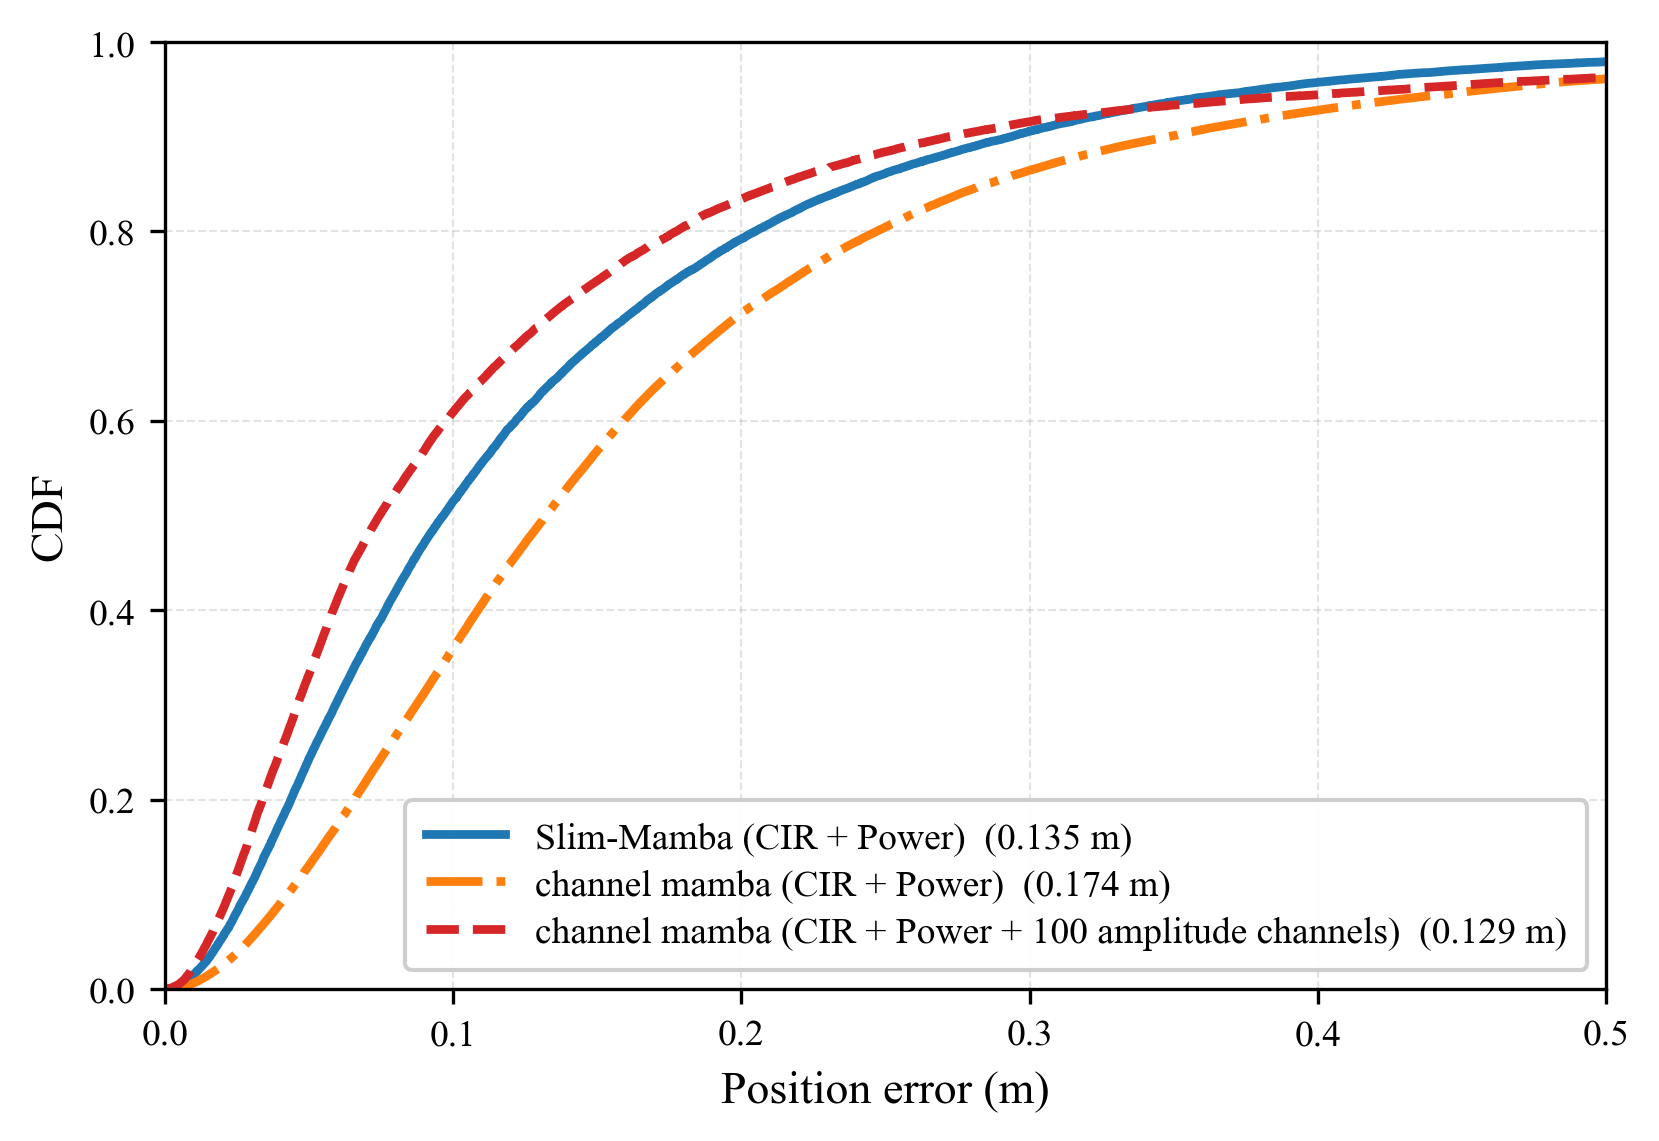
\includegraphics[width=0.68\linewidth]{generated_figures/software_eval_model_comparison_cdf.png}
  \caption{Cumulative distribution of localization error for Slim-Mamba and two channel mamba reference runs under matched and augmented input settings.}
  \label{fig:cdf_zoom}
\end{figure}

\begin{figure}[H]
  \centering
  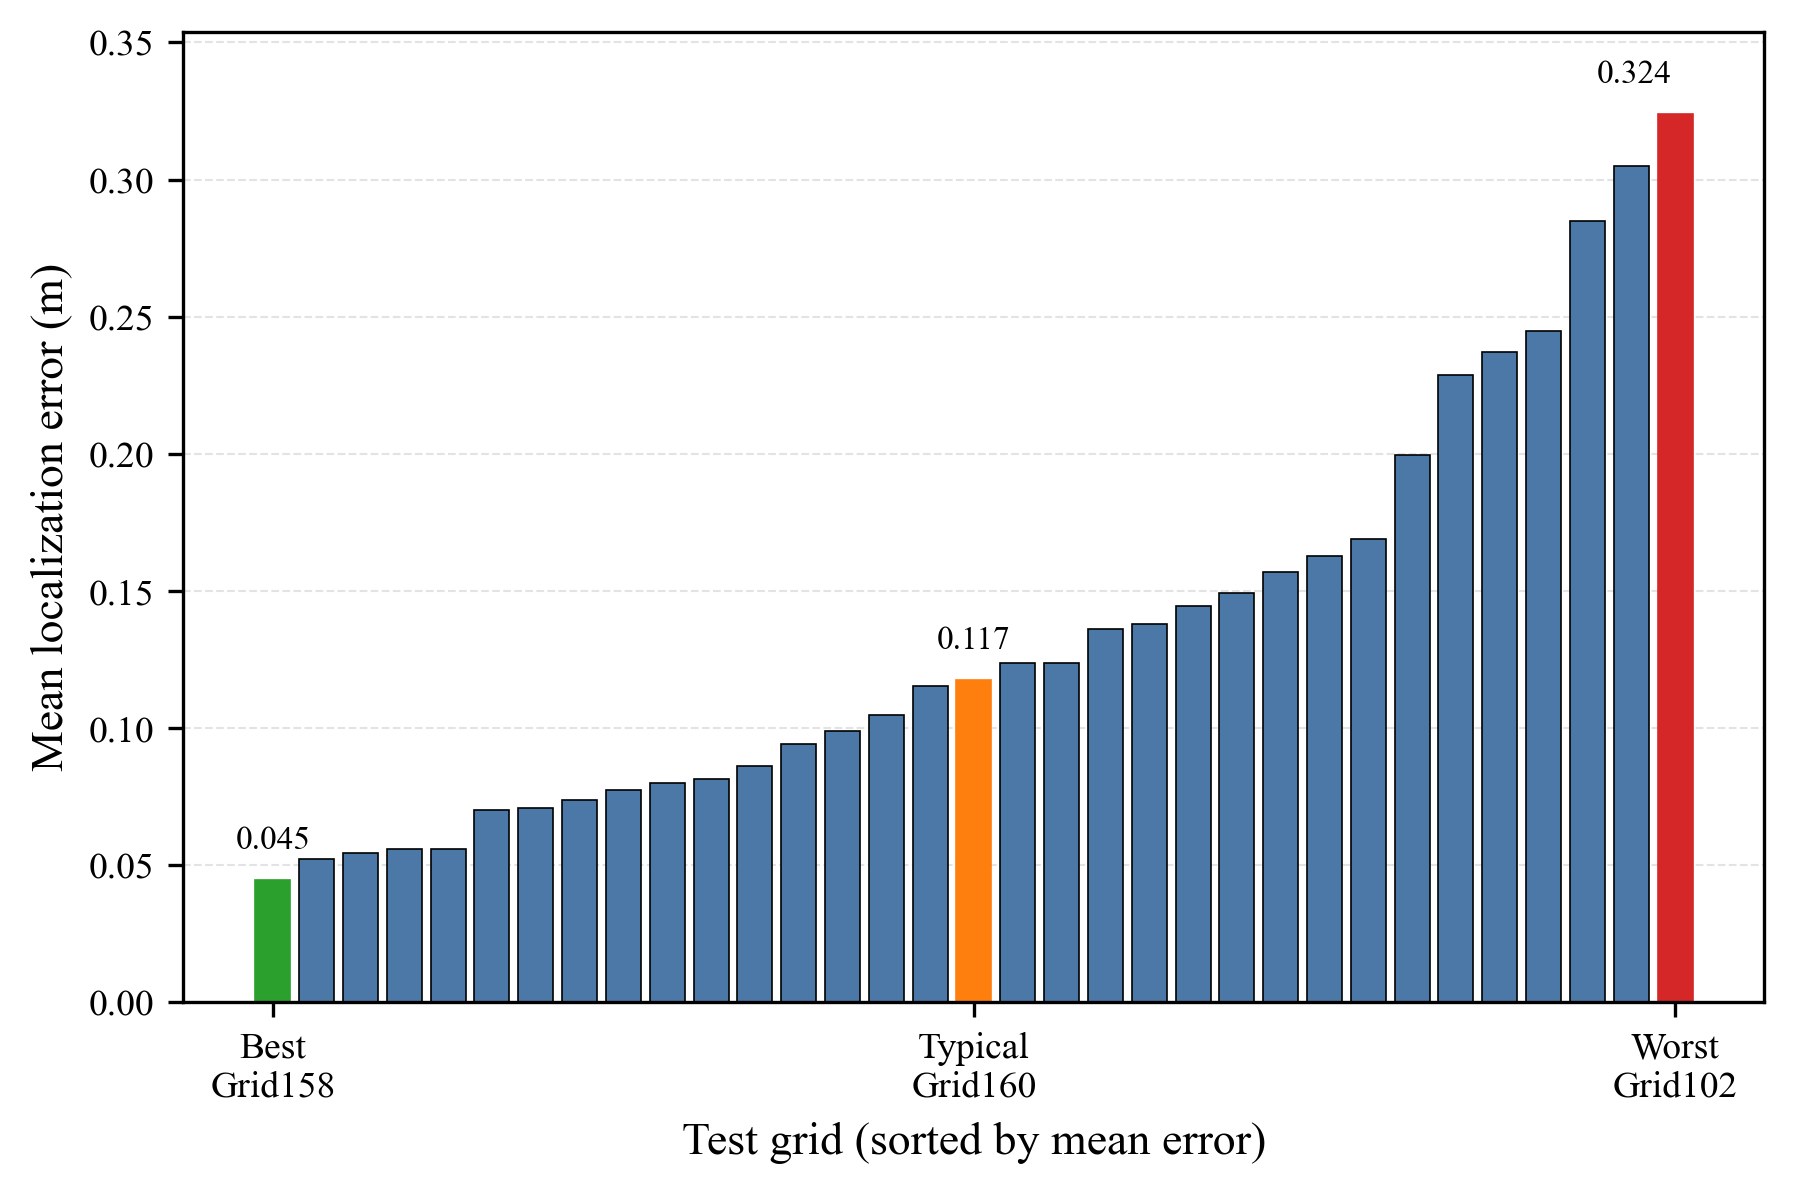
\includegraphics[width=0.88\linewidth]{generated_figures/software_eval_slim_grid_ranking.png}
  \caption{Per-grid mean localization error of the final Slim-Mamba model on the test set, sorted from best to worst.}
  \label{fig:slim_grid_ranking}
\end{figure}

The grid-level ranking in Fig.~\ref{fig:slim_grid_ranking} shows that the final
Slim-Mamba model maintains a stable error level over most of the test set, while the
remaining variation across grids is correlated with the local trajectory coverage around
each query position. When a test trajectory lies in a region that is surrounded by more
training trajectories, the localization error is generally lower; when the nearby
trajectory coverage becomes sparser, the error tends to increase. Therefore,
Fig.~\ref{fig:software_eval_panel} presents representative examples from the low-error,
mid-error, and high-error parts of the ranking to illustrate this spatial trend on the
test set.

\begin{figure}[H]
  \centering
  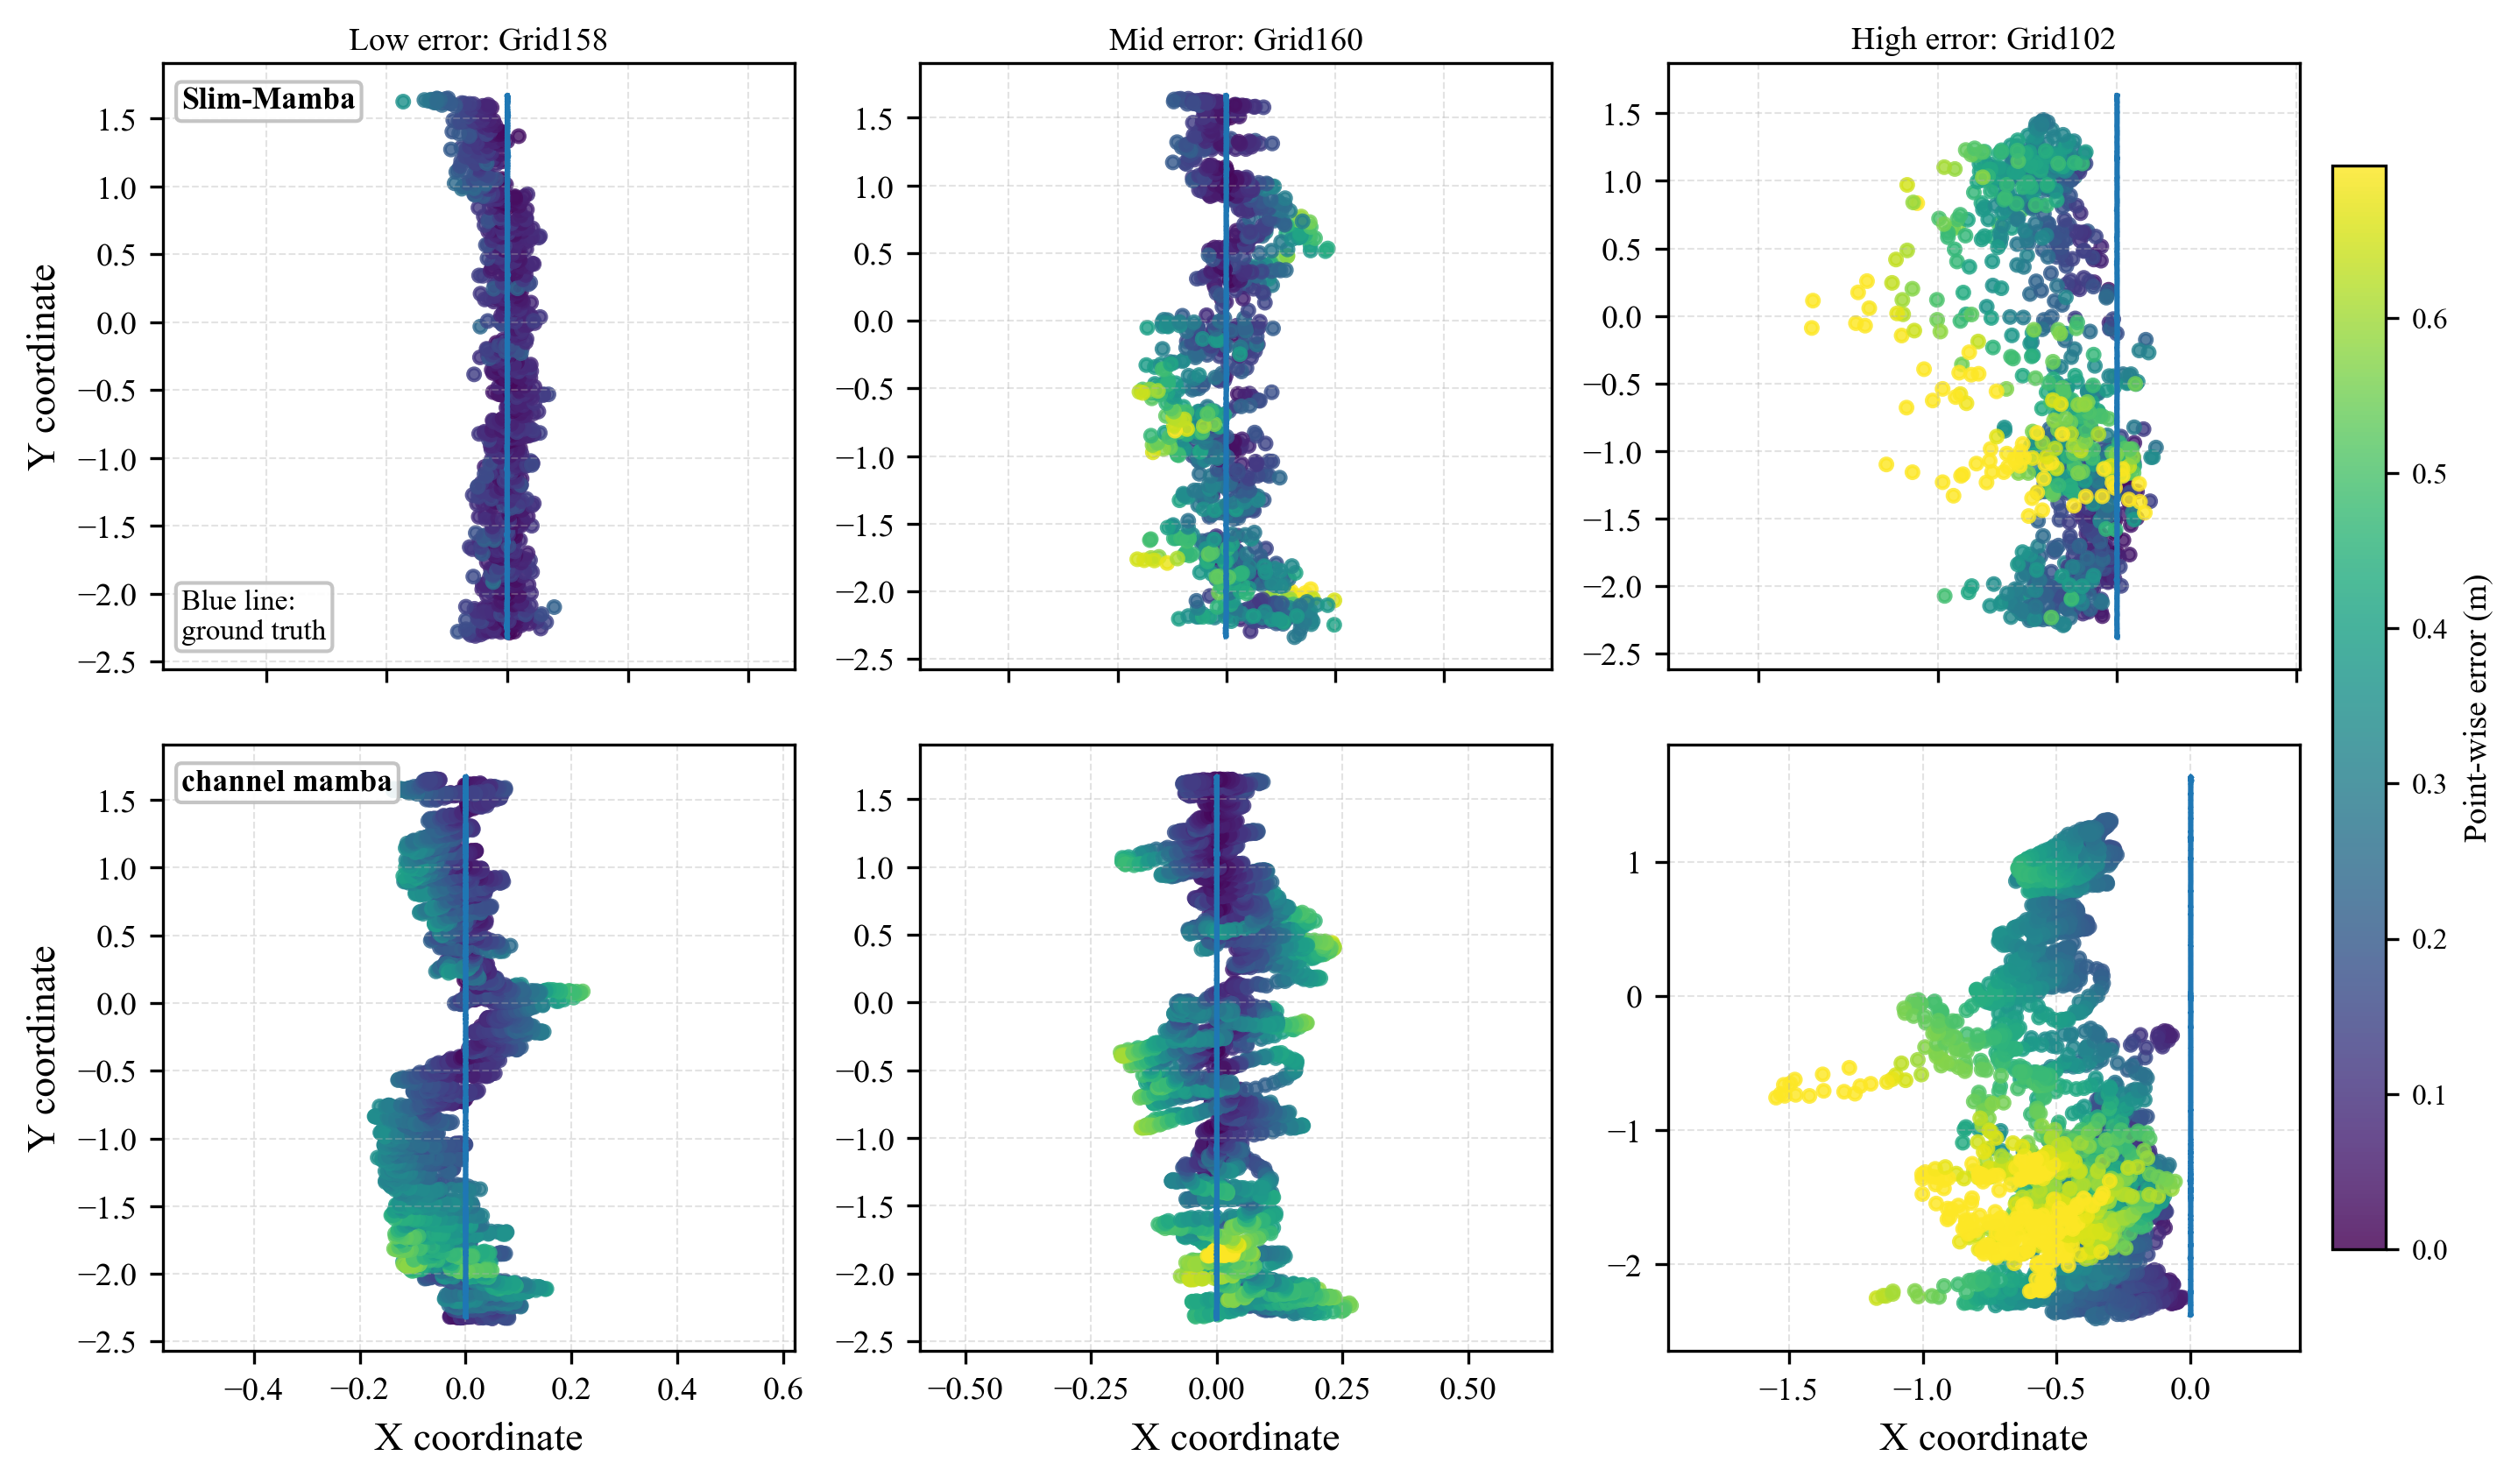
\includegraphics[width=0.94\linewidth]{generated_figures/software_eval_best_typical_worst_panel.png}
  \caption{Trajectory-level comparisons on low-, mid-, and high-error grids for Slim-Mamba (top) and channel mamba (bottom).}
  \label{fig:software_eval_panel}
\end{figure}

After selecting Slim-Mamba as the deployment-oriented model, the temporal window length
\(K\) and patch setting are ablated. Table~\ref{tab:k_ablation} shows that \(K=1\) and
\(K=2\) both achieve the best test mean error of about 0.135~m, while longer temporal
windows gradually increase the test error. The CDF comparison in
Fig.~\ref{fig:k_ablation_cdf} shows the same trend from a distributional perspective:
short-window configurations keep more samples in the low-error region, whereas larger
\(K\) values mainly broaden the error tail. This suggests that, under the current LuViRA
sampling density, extending the temporal context introduces more redundancy than useful
additional localization cues. Therefore, short-window Slim-Mamba is used as the software
model target for the subsequent hardware implementation.

\begin{figure}[H]
  \centering
  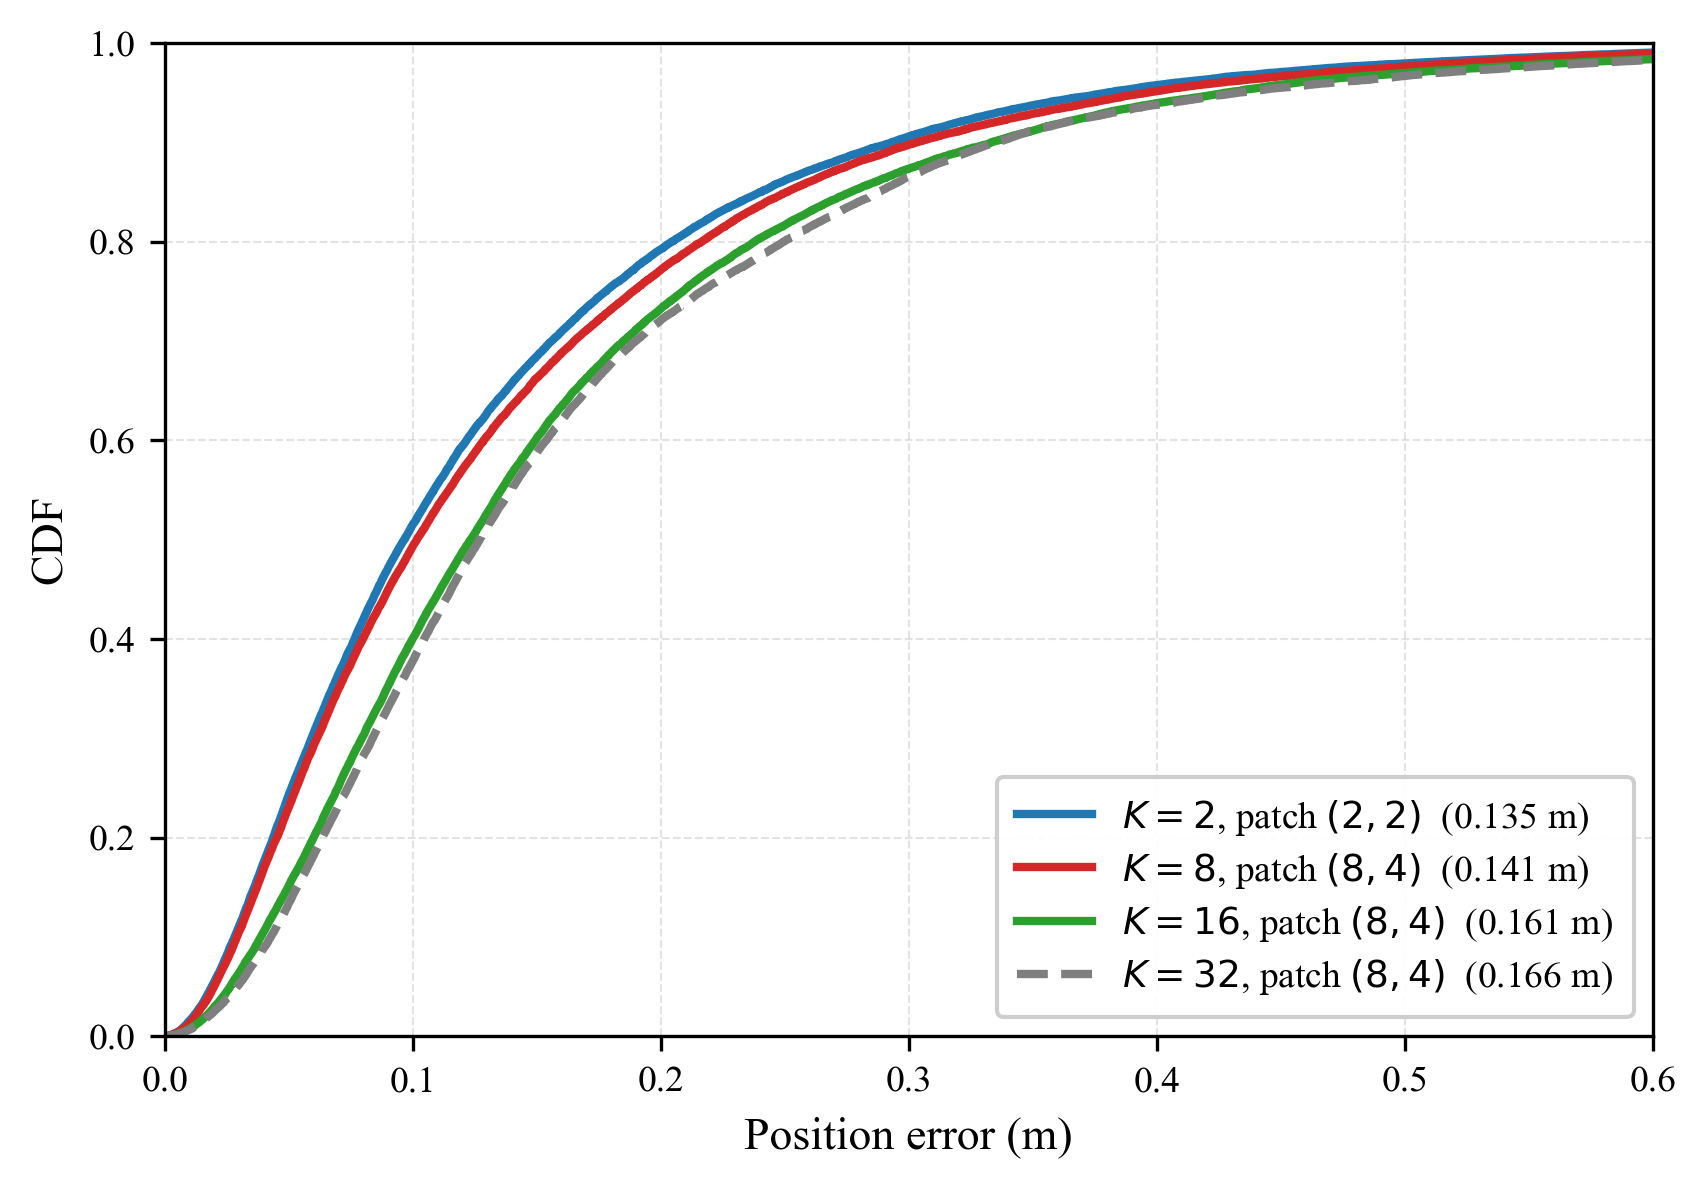
\includegraphics[width=0.78\linewidth]{generated_figures/software_eval_k_ablation_cdf.png}
  \caption{Cumulative distribution of localization error for representative Slim-Mamba temporal-window configurations.}
  \label{fig:k_ablation_cdf}
\end{figure}

\begin{table}[H]
\centering
\caption{Ablation on window length \(K\) with patch length and stride variants.}
\label{tab:k_ablation}
\footnotesize
\setlength{\tabcolsep}{5pt}
\renewcommand{\arraystretch}{1.12}
\begin{tabular}{c c c}
\hline
\textbf{\(K\) (patch length, stride)} & \textbf{Eval mean err. (m)} &
\textbf{Test mean err. (m)} \\
\hline
1  (1,1) & 0.10068 & \textbf{0.135} \\
2  (2,2) & 0.09557 & \textbf{0.135} \\
4  (2,2) & 0.09814 & 0.139 \\
8  (2,2) & 0.09405 & 0.141 \\
4  (4,4) & 0.09983 & 0.137 \\
6  (4,4) & 0.09839 & 0.138 \\
8  (4,4) & 0.09749 & 0.144 \\
8  (8,4) & 0.09744 & 0.152 \\
12 (8,4) & 0.09286 & 0.156 \\
16 (8,4) & 0.09225 & 0.161 \\
24 (8,4) & 0.09432 & 0.159 \\
32 (8,4) & 0.09328 & 0.166 \\
\hline
\end{tabular}
\end{table}

\section{Accuracy}

This section evaluates the localization accuracy across three stages: the
floating-point Slim-Mamba model, the fake-quantized model, and the hardware fixed-point
model. The floating-point model is used as the software reference. The fake-quantized
model inserts quantize and dequantize operations during software inference and is used
to evaluate the effect of the selected bit-widths. The hardware fixed-point model
further follows the integer datapath used in RTL, including fixed-point multiplication,
shifting, rounding, saturation, lookup-table nonlinear functions, and dynamic scaling in
the selective-scan state path. This layered comparison separates the model accuracy,
software quantization error, and hardware fixed-point mapping error.

\begin{table}[H]
\centering
\caption{Accuracy comparison across floating-point, fake-quantized, and hardware fixed-point models.}
\label{tab:accuracy_eval}
\small
\setlength{\tabcolsep}{5pt}
\resizebox{\linewidth}{!}{%
\begin{tabular}{l c c c}
\hline
\textbf{Model stage} & \textbf{Numerical format} & \textbf{Output MAE vs. float} &
\textbf{Mean localization error (m)} \\
\hline
Floating-point Slim-Mamba & Float32 & -- & 0.13500 \\
Fake-quantized Slim-Mamba & Software fake quant & -- & 0.13695 \\
Hardware fixed-point model & Fixed-point with dynamic scale & 0.02081 & 0.14103 \\
\hline
\end{tabular}%
}
\end{table}

Table~\ref{tab:accuracy_eval} shows that fake quantization introduces almost no
additional localization error compared with the floating-point Slim-Mamba model. This
indicates that the unified 16-bit datapath and the selected Q formats are sufficient for
the main computation paths. The hardware fixed-point model increases the mean
localization error from 0.13500~m to 0.14103~m. It also gives an output MAE of 0.02081
with respect to the floating-point output. This confirms that fixed-point arithmetic
does introduce numerical differences, but these differences are not strongly amplified
in the final localization result.

The main accuracy loss therefore comes from the hardware fixed-point mapping stage
rather than from the software fake-quantization stage. This is expected because the
hardware fixed-point model includes concrete RTL-oriented numerical behavior, such as
round-to-nearest-even, saturation clamp, LUT-based nonlinear approximation, fixed-point
scale multiplication, and dynamic scaling for the selective-scan state. Nevertheless,
the final mean localization error remains below 0.15~m and is only about 0.006~m higher
than the floating-point result. This validates the quantization strategy described in
Section~\ref{subsec:quant_error_strategy}, including the unified 16-bit datapath,
Q8.8/Q0.16/Q1.15 formats, saturation handling, and selective-scan dynamic scaling.

\section{Performance}

This section evaluates the FPGA accelerator in terms of throughput, resource
utilization, power, and block-level latency. The target real-time requirement is
100~frames/s. The implemented design closes timing at 100~MHz and achieves an estimated
throughput of 471~frames/s, which is about \(4.7\times\) higher than the requirement.
This corresponds to an average processing time of about 2.12~ms per frame, compared with
the 10~ms frame interval allowed by the target requirement.

\begin{table}[H]
\caption{Throughput summary at 100~MHz.}
\label{tab:throughput_summary}
\centering
\small
\begin{tabular}{l c}
\hline
\textbf{Metric} & \textbf{Value} \\
\hline
Target clock frequency & 100~MHz \\
Required throughput & 100~frames/s \\
Achieved throughput & 471~frames/s \\
Average time per frame & 2.12~ms \\
Requirement time per frame & 10~ms \\
\hline
\end{tabular}
\end{table}

Table~\ref{tab:resource_utilization} reports the post-synthesis resource utilization
under the 100~MHz constraint. The design uses 22.21\% of LUTs, 14.11\% of flip-flops,
30.59\% of BRAM tiles, and 19.68\% of DSP blocks. The BRAM usage mainly comes from
on-chip weight memories, intermediate buffers, state SRAM, and lookup tables. The DSP
usage is dominated by the shared MAC fabric, RMSNorm, element-wise multiplication, and
scale-related fixed-point multiplications. Overall, the utilization remains well below
the device capacity, leaving room for further optimization or model scaling.

\begin{table}[H]
\caption{Post-synthesis resource utilization at 100~MHz.}
\label{tab:resource_utilization}
\centering
\small
\begin{tabular}{l c c c}
\hline
\textbf{Resource} & \textbf{Used} & \textbf{Available} & \textbf{Utilization} \\
\hline
LUT & 60868 & 274080 & 22.21\% \\
FF & 77345 & 548160 & 14.11\% \\
BRAM tiles & 279 & 912 & 30.59\% \\
DSP & 496 & 2520 & 19.68\% \\
Bonded IOB & 0 & 328 & 0\% \\
\hline
\end{tabular}
\end{table}

The on-chip power estimate is summarized in Table~\ref{tab:power_summary}. The total
on-chip power is 4.292~W, including 3.562~W dynamic power and 0.729~W static power. The
processing system contributes 2.622~W of the dynamic power, which is about 74\% of the
dynamic component. This indicates that the total system power is not only determined by
the programmable logic compute array, but also by the PS-side control, DDR access, and
DMA-based data movement.

\begin{table}[H]
\caption{On-chip power estimate.}
\label{tab:power_summary}
\centering
\small
\begin{tabular}{l c c}
\hline
\textbf{Power item} & \textbf{Power} & \textbf{Share} \\
\hline
Total on-chip power & 4.292~W & 100\% \\
Dynamic power & 3.562~W & 83\% \\
Static power & 0.729~W & 17\% \\
PS dynamic power & 2.622~W & 74\% of dynamic power \\
\hline
\end{tabular}
\end{table}

Before optimizing the hardware schedule, a function-level profiling study is used to
identify the dominant computation. As shown in Table~\ref{tab:ssm_profile}, the SSM
path is the most important part of the workload. The SSM \(dt\) projection accounts for
36.18\% of the profiled time, and the selective-scan state update accounts for 41.34\%.
Together, they contribute more than 77\% of the listed execution time. This motivates
the fine-grained pipeline design for the SSM path, since improving this part has the
largest impact on the end-to-end block latency.

\begin{table}[H]
\caption{Function-level profiling summary.}
\label{tab:ssm_profile}
\centering
\scriptsize
\begin{tabular}{l|c|c}
\hline
\textbf{Function} & \textbf{Time} & \textbf{Share (\%)} \\
\hline
Linear projection (in/out)         & 30  & 7.75  \\
Normalization (RMSNorm)            & 57  & 14.73 \\
SSM \(dt\) projection (MVM + sigmoid) & 140 & 36.18 \\
SSM selective scan (state update)  & 160 & 41.34 \\
\hline
Total (listed)                     & 387 & 100.00 \\
\hline
\end{tabular}
\end{table}

Table~\ref{tab:block_latency} gives the per-block latency breakdown. The total latency
of one Slim-Mamba block is 5301 cycles, or 53.01~\(\mu\)s at 100~MHz. Input projection
takes 2305 cycles, while the complete SSM part takes 1828 cycles. These two parts are
useful for comparison because their main projection workloads have the same theoretical
number of MAC operations. In the RTL configuration, the input projection maps a
128-dimensional vector to a 512-dimensional output, corresponding to
\(128 \times 512 = 65{,}536\) MAC operations. The SSM \(dt\) projection maps a
256-dimensional vector to a 256-dimensional vector, also corresponding to
\(256 \times 256 = 65{,}536\) MAC operations. However, the SSM path also includes
sigmoid generation, selective-scan state update, element-wise operations, and scale
alignment. Even with these extra operations, the SSM latency remains lower than the
input-projection latency. This is mainly due to the fine-grained FIFO-based pipeline:
the \(dt\) projection output is forwarded to the selective-scan and gating-related
stages at tile granularity, instead of waiting for the full vector to be generated.

\begin{table}[H]
\caption{Latency breakdown per Slim-Mamba block.}
\label{tab:block_latency}
\centering
\small
\begin{tabular}{l c c}
\hline
\textbf{Category} & \textbf{Clock cycles} & \textbf{Share} \\
\hline
RMSNorm & 134 & 2.5\% \\
Input projection & 2305 & 47.25\% \\
Ping-pong buffer & 199 & 3.75\% \\
SSM & 1828 & 34.48\% \\
Output projection & 833 & 15.71\% \\
\hline
Total & 5301 & 100\% \\
\hline
\end{tabular}
\end{table}

Overall, the accelerator satisfies the real-time throughput target with a large margin
while keeping resource utilization moderate. The profiling and latency results also
confirm the effectiveness of the SSM fine-grained pipeline: the most critical software
workload is mapped to a streaming hardware schedule that reduces waiting time between
the projection, nonlinear, and state-update stages.

\section{FPGA On-board Validation}

The final step is to validate that the FPGA platform can execute the complete hardware
path on board. The purpose of this test is not to run the full LuViRA test set, but to
confirm that the processing system, DDR buffers, AXI DMA channels, AXI-Lite control
registers, stream loader, four-block compute chain, and output write-back path are all
connected correctly. The validation flow is shown in Fig.~\ref{fig:board_validate}.

\begin{figure}[H]
  \centering
  \includesvg[inkscapelatex=false,width=0.75\linewidth]{board_validate}
  \caption{FPGA on-board validation flow.}
  \label{fig:board_validate}
\end{figure}

In the current bring-up experiment, the SD card boot and model-file loading path is not
used as part of the test. Instead, the host-side program prepares a large input matrix
file containing a subset of validation samples. This matrix is loaded by the processing
system into the DDR input buffer. The PS then programs the AXI DMA and the AXI-Lite
control registers, starts the input preload and computation sequence, and waits for the
completion status from the PL. During execution, the MM2S DMA channel streams the input
matrix from DDR to the PL, and the board shell feeds the data into the four-block
Slim-Mamba chain. After computation, the S2MM DMA channel writes the output stream back
to the DDR output buffer, where it is read by the host-side program for checking.

The on-board test uses only a partial dataset, so it should be interpreted as a platform
validation rather than a full accuracy evaluation. Nevertheless, the test passes with
the expected completion status and output transfer behavior. This confirms that the
main FPGA platform components are functional as an integrated system: PS-side control,
DDR buffering, AXI-Lite register access, AXI DMA streaming, PL-side input loading,
four-block computation, and output write-back are all exercised in one run. Therefore,
the current result demonstrates that the accelerator has been successfully brought up on
the FPGA platform.
\chapter{Conclusion}

\section{Conclusion}

This thesis investigated the use of Mamba-family models for Massive MIMO indoor
localization and developed a hardware-oriented Slim-Mamba accelerator on FPGA. The work
combined software evaluation, fixed-point quantization, and RTL implementation. Based
on LuViRA experiments, Slim-Mamba was selected as a deployment-oriented model because it
keeps the recurrent update and gating behavior needed for localization while avoiding
unnecessary multi-branch fusion and full selective-scan complexity.

The accelerator was implemented on a Zynq MPSoC platform with PS-side DDR/DMA control
and a PL-side four-block Slim-Mamba compute chain. The design uses a shared
\(4\times4\times4\) MAC fabric, hardware nonlinear units, configurable quantization
modules, and a dynamic-scale state path. The hardware fixed-point model reaches a mean
localization error of 0.14103~m, close to the floating-point result of 0.13500~m. The
RTL design closes timing at 100~MHz and achieves 471~frames/s, exceeding the
100~frames/s requirement, while reconfigurable MAC architecture keeps a low utilization
(22.21\% LUTs, 14.11\% FFs, 30.59\% BRAM tiles, and
19.68\% DSPs). Board-level validation confirms that PS control, DDR buffering, AXI DMA
streaming, PL computation, and output write-back are connected and functional.

\section{Future Work}

Although the current design demonstrates the feasibility of a Slim-Mamba FPGA
accelerator, several directions remain for future work.

\begin{itemize}
  \item \textbf{Full end-to-end board evaluation:} The current on-board validation uses a
  partial input matrix and does not yet use SD-card model loading. Future work should run
  the full LuViRA set on board and integrate model loading, DDR buffer preparation, and
  output checking.

  \item \textbf{Finer-grained whole-architecture pipeline:} In the current design, the SSM
  path is fine-grained, while RMSNorm, input projection, output projection, residual
  preload, and block-level scheduling still use coarser boundaries. These stages can be
  further overlapped to reduce end-to-end latency.

\end{itemize}

%%%%%%%%%%%%%%%%%%%%%%%%%%%%%%%%%%%%%%%
%% References
\begin{thebibliography}{99}
\bibitem{cite:Bourdoux2020} A. Bourdoux, A. N. Barreto, B. Van Liempd, et al., ``6G white paper on localization and sensing,'' arXiv preprint arXiv:2006.01779, 2020.
\bibitem{cite:Trevlakis2023} S. E. Trevlakis, A. A. A. Boulogeorgos, D. Pliatsios, et al., ``Localization as a key enabler of 6G wireless systems: A comprehensive survey and an outlook,'' \textit{IEEE Open Journal of the Communications Society}, 2023.
\bibitem{cite:Mogyorosi2022} F. Mogyor\'osi, P. Revisnyei, A. Pa\v{s}i\'c, et al., ``Positioning in 5G and 6G networks---A survey,'' \textit{Sensors}, vol. 22, no. 13, p. 4757, 2022.
\bibitem{cite:Tian2024} G. Tian, I. Yaman, M. Sandra, et al., ``Deep-learning-based high-precision localization with Massive MIMO,'' \textit{IEEE Transactions on Machine Learning in Communications and Networking}, vol. 2, pp. 19--34, 2024.
\bibitem{cite:TianICC2023} G. Tian, I. Yaman, M. Sandra, et al., ``High-precision machine-learning based indoor localization with Massive MIMO system,'' in \textit{ICC 2023 --- IEEE International Conference on Communications}, Rome, Italy, 2023, pp. 3690--3695.
\bibitem{cite:LuViRA2024} I. Yaman, G. Tian, M. Larsson, P. Persson, M. Sandra, A. D\"urr, E. Tegler, N. Challa, H. Garde, F. Tufvesson, K. \AA str\"om, O. Edfors, S. Malkowsky, and L. Liu, ``The LuViRA Dataset: Synchronized vision, radio, and audio sensors for indoor localization,'' in \textit{2024 IEEE International Conference on Robotics and Automation (ICRA)}, 2024, pp. 11920--11926, doi: 10.1109/ICRA57147.2024.10610237.
\bibitem{cite:Colpaert2023} A. Colpaert, S. De Bast, R. Beerten, A. P. Guevara, Z. Cui, and S. Pollin, ``Massive MIMO channel measurement data set for localization and communication,'' \textit{IEEE Communications Magazine}, vol. 61, no. 9, pp. 114--120, Sep. 2023.
\bibitem{cite:Cunningham2022KNN} P. Cunningham and S. J. Delany, ``K-nearest neighbour classifiers---A tutorial,'' \textit{ACM Computing Surveys}, vol. 54, no. 6, pp. 1--25, Jul. 2022.
\bibitem{cite:Yaro2023} A. S. Yaro, F. Maly, and P. Prazak, ``A survey of the performance-limiting factors of a 2-dimensional RSS fingerprinting-based indoor wireless localization system,'' \textit{Sensors}, vol. 23, no. 5, p. 2545, 2023.
\bibitem{cite:Mamba2023} A. Gu and T. Dao, ``Mamba: Linear-time sequence modeling with selective state spaces,'' arXiv preprint arXiv:2312.00752, 2023.
\bibitem{cite:CMamba2024} C. Zeng, Z. Liu, G. Zheng, and L. Kong, ``CMamba: Channel correlation enhanced state space models for multivariate time series forecasting,'' arXiv preprint arXiv:2406.05316, 2024.
\bibitem{cite:LightMamba2025} R. Wei, S. Xu, L. Zhong, et al., ``LightMamba: Efficient Mamba acceleration on FPGA with quantization and hardware co-design,'' in \textit{2025 Design, Automation \& Test in Europe Conference (DATE)}, IEEE, 2025. Available: \url{https://arxiv.org/abs/2502.15260}.
\bibitem{cite:FastMamba2025} A. Wang, H. Shao, S. Ma, et al., ``FastMamba: A high-speed and efficient Mamba accelerator on FPGA with accurate quantization,'' arXiv preprint arXiv:2505.18975, 2025. Available: \url{https://arxiv.org/abs/2505.18975}.
\bibitem{cite:HCSA2025} X. Jin, H. Zheng, M. Nie, et al., ``HCSAs: Hybrid computing systolic arrays for accelerating Mamba models with unified state space buffers and energy-efficient dataflow,'' in \textit{Great Lakes Symposium on VLSI 2025}, New York: ACM, 2025, pp. 457--462, doi: 10.1145/3716368.3735187.
\bibitem{cite:Sutikno2014Sqrt} T. Sutikno, A. Z. Jidin, A. Jidin, and N. R. N. Idris, ``Strategies for FPGA implementation of non-restoring square root algorithm,'' \textit{International Journal of Electrical \& Computer Engineering}, 2014.
\bibitem{cite:Istoan2015ReciprocalSqrt} M. Istoan and B. Pasca, ``Fixed-point implementations of the reciprocal, square root and reciprocal square root functions,'' 2015. Available: \url{https://hal.science/hal-01229538}.
\end{thebibliography}


%%%%%%%%%%%%%%%%%%
\appendix
%%%%%%%%%%%%%%%%%%
\chapter{Some extra material}
\lipsum[1]
\begin{figure}[htbp]
  \centering
  \includegraphics[width=0.6\linewidth]{example-image}
  \caption{A picture or table in the appendix is numbered accordingly.}
  \label{fig:AppFig}
\end{figure}

\end{document}
